\documentclass[twoside]{book}

% Packages required by doxygen
\usepackage{fixltx2e}
\usepackage{calc}
\usepackage{doxygen}
\usepackage[export]{adjustbox} % also loads graphicx
\usepackage{graphicx}
\usepackage[utf8]{inputenc}
\usepackage{makeidx}
\usepackage{multicol}
\usepackage{multirow}
\PassOptionsToPackage{warn}{textcomp}
\usepackage{textcomp}
\usepackage[nointegrals]{wasysym}
\usepackage[table]{xcolor}

% Font selection
\usepackage[T1]{fontenc}
\usepackage[scaled=.90]{helvet}
\usepackage{courier}
\usepackage{amssymb}
\usepackage{sectsty}
\renewcommand{\familydefault}{\sfdefault}
\allsectionsfont{%
  \fontseries{bc}\selectfont%
  \color{darkgray}%
}
\renewcommand{\DoxyLabelFont}{%
  \fontseries{bc}\selectfont%
  \color{darkgray}%
}
\newcommand{\+}{\discretionary{\mbox{\scriptsize$\hookleftarrow$}}{}{}}

% Page & text layout
\usepackage{geometry}
\geometry{%
  a4paper,%
  top=2.5cm,%
  bottom=2.5cm,%
  left=2.5cm,%
  right=2.5cm%
}
\tolerance=750
\hfuzz=15pt
\hbadness=750
\setlength{\emergencystretch}{15pt}
\setlength{\parindent}{0cm}
\setlength{\parskip}{3ex plus 2ex minus 2ex}
\makeatletter
\renewcommand{\paragraph}{%
  \@startsection{paragraph}{4}{0ex}{-1.0ex}{1.0ex}{%
    \normalfont\normalsize\bfseries\SS@parafont%
  }%
}
\renewcommand{\subparagraph}{%
  \@startsection{subparagraph}{5}{0ex}{-1.0ex}{1.0ex}{%
    \normalfont\normalsize\bfseries\SS@subparafont%
  }%
}
\makeatother

% Headers & footers
\usepackage{fancyhdr}
\pagestyle{fancyplain}
\fancyhead[LE]{\fancyplain{}{\bfseries\thepage}}
\fancyhead[CE]{\fancyplain{}{}}
\fancyhead[RE]{\fancyplain{}{\bfseries\leftmark}}
\fancyhead[LO]{\fancyplain{}{\bfseries\rightmark}}
\fancyhead[CO]{\fancyplain{}{}}
\fancyhead[RO]{\fancyplain{}{\bfseries\thepage}}
\fancyfoot[LE]{\fancyplain{}{}}
\fancyfoot[CE]{\fancyplain{}{}}
\fancyfoot[RE]{\fancyplain{}{\bfseries\scriptsize Generated by Doxygen }}
\fancyfoot[LO]{\fancyplain{}{\bfseries\scriptsize Generated by Doxygen }}
\fancyfoot[CO]{\fancyplain{}{}}
\fancyfoot[RO]{\fancyplain{}{}}
\renewcommand{\footrulewidth}{0.4pt}
\renewcommand{\chaptermark}[1]{%
  \markboth{#1}{}%
}
\renewcommand{\sectionmark}[1]{%
  \markright{\thesection\ #1}%
}

% Indices & bibliography
\usepackage{natbib}
\usepackage[titles]{tocloft}
\setcounter{tocdepth}{3}
\setcounter{secnumdepth}{5}
\makeindex

% Hyperlinks (required, but should be loaded last)
\usepackage{ifpdf}
\ifpdf
  \usepackage[pdftex,pagebackref=true]{hyperref}
\else
  \usepackage[ps2pdf,pagebackref=true]{hyperref}
\fi
\hypersetup{%
  colorlinks=true,%
  linkcolor=blue,%
  citecolor=blue,%
  unicode%
}

% Custom commands
\newcommand{\clearemptydoublepage}{%
  \newpage{\pagestyle{empty}\cleardoublepage}%
}

\usepackage{caption}
\captionsetup{labelsep=space,justification=centering,font={bf},singlelinecheck=off,skip=4pt,position=top}

%===== C O N T E N T S =====

\begin{document}

% Titlepage & ToC
\hypersetup{pageanchor=false,
             bookmarksnumbered=true,
             pdfencoding=unicode
            }
\pagenumbering{roman}
\begin{titlepage}
\vspace*{7cm}
\begin{center}%
{\Large Ray\+Tracing }\\
\vspace*{1cm}
{\large Generated by Doxygen 1.8.11}\\
\end{center}
\end{titlepage}
\clearemptydoublepage
\tableofcontents
\clearemptydoublepage
\pagenumbering{arabic}
\hypersetup{pageanchor=true}

%--- Begin generated contents ---
\chapter{Hierarchical Index}
\section{Class Hierarchy}
This inheritance list is sorted roughly, but not completely, alphabetically\+:\begin{DoxyCompactList}
\item \contentsline{section}{Camera}{\pageref{class_camera}}{}
\item \contentsline{section}{Collision\+Point}{\pageref{class_collision_point}}{}
\item \contentsline{section}{J\+S\+O\+N\+Parser}{\pageref{class_j_s_o_n_parser}}{}
\item \contentsline{section}{Light}{\pageref{class_light}}{}
\item \contentsline{section}{Lode\+P\+N\+G\+Color\+Mode}{\pageref{struct_lode_p_n_g_color_mode}}{}
\item \contentsline{section}{Lode\+P\+N\+G\+Color\+Profile}{\pageref{struct_lode_p_n_g_color_profile}}{}
\item \contentsline{section}{Lode\+P\+N\+G\+Compress\+Settings}{\pageref{struct_lode_p_n_g_compress_settings}}{}
\item \contentsline{section}{Lode\+P\+N\+G\+Decoder\+Settings}{\pageref{struct_lode_p_n_g_decoder_settings}}{}
\item \contentsline{section}{Lode\+P\+N\+G\+Decompress\+Settings}{\pageref{struct_lode_p_n_g_decompress_settings}}{}
\item \contentsline{section}{Lode\+P\+N\+G\+Encoder\+Settings}{\pageref{struct_lode_p_n_g_encoder_settings}}{}
\item \contentsline{section}{Lode\+P\+N\+G\+Info}{\pageref{struct_lode_p_n_g_info}}{}
\item \contentsline{section}{Lode\+P\+N\+G\+State}{\pageref{struct_lode_p_n_g_state}}{}
\item \contentsline{section}{Lode\+P\+N\+G\+Time}{\pageref{struct_lode_p_n_g_time}}{}
\item \contentsline{section}{P\+N\+G\+Renderer}{\pageref{class_p_n_g_renderer}}{}
\item \contentsline{section}{Ray}{\pageref{class_ray}}{}
\item \contentsline{section}{Raytracer}{\pageref{class_raytracer}}{}
\item \contentsline{section}{Scene}{\pageref{class_scene}}{}
\item \contentsline{section}{S\+Hape}{\pageref{class_s_hape}}{}
\item \contentsline{section}{Shape}{\pageref{class_shape}}{}
\begin{DoxyCompactList}
\item \contentsline{section}{Box}{\pageref{class_box}}{}
\item \contentsline{section}{Sphere}{\pageref{class_sphere}}{}
\end{DoxyCompactList}
\end{DoxyCompactList}

\chapter{Class Index}
\section{Class List}
Here are the classes, structs, unions and interfaces with brief descriptions\+:\begin{DoxyCompactList}
\item\contentsline{section}{\hyperlink{class_box}{Box} \\*Class representing a box in the scene }{\pageref{class_box}}{}
\item\contentsline{section}{\hyperlink{class_camera}{Camera} \\*Class representing a camera }{\pageref{class_camera}}{}
\item\contentsline{section}{\hyperlink{class_collision_point}{Collision\+Point} \\*Class representing a collision point }{\pageref{class_collision_point}}{}
\item\contentsline{section}{\hyperlink{class_j_s_o_n_parser}{J\+S\+O\+N\+Parser} \\*Helper class to parse the J\+S\+ON scene files }{\pageref{class_j_s_o_n_parser}}{}
\item\contentsline{section}{\hyperlink{class_light}{Light} \\*Class representing a light in the scene }{\pageref{class_light}}{}
\item\contentsline{section}{\hyperlink{struct_lode_p_n_g_color_mode}{Lode\+P\+N\+G\+Color\+Mode} }{\pageref{struct_lode_p_n_g_color_mode}}{}
\item\contentsline{section}{\hyperlink{struct_lode_p_n_g_color_profile}{Lode\+P\+N\+G\+Color\+Profile} }{\pageref{struct_lode_p_n_g_color_profile}}{}
\item\contentsline{section}{\hyperlink{struct_lode_p_n_g_compress_settings}{Lode\+P\+N\+G\+Compress\+Settings} }{\pageref{struct_lode_p_n_g_compress_settings}}{}
\item\contentsline{section}{\hyperlink{struct_lode_p_n_g_decoder_settings}{Lode\+P\+N\+G\+Decoder\+Settings} }{\pageref{struct_lode_p_n_g_decoder_settings}}{}
\item\contentsline{section}{\hyperlink{struct_lode_p_n_g_decompress_settings}{Lode\+P\+N\+G\+Decompress\+Settings} }{\pageref{struct_lode_p_n_g_decompress_settings}}{}
\item\contentsline{section}{\hyperlink{struct_lode_p_n_g_encoder_settings}{Lode\+P\+N\+G\+Encoder\+Settings} }{\pageref{struct_lode_p_n_g_encoder_settings}}{}
\item\contentsline{section}{\hyperlink{struct_lode_p_n_g_info}{Lode\+P\+N\+G\+Info} }{\pageref{struct_lode_p_n_g_info}}{}
\item\contentsline{section}{\hyperlink{struct_lode_p_n_g_state}{Lode\+P\+N\+G\+State} }{\pageref{struct_lode_p_n_g_state}}{}
\item\contentsline{section}{\hyperlink{struct_lode_p_n_g_time}{Lode\+P\+N\+G\+Time} }{\pageref{struct_lode_p_n_g_time}}{}
\item\contentsline{section}{\hyperlink{class_p_n_g_renderer}{P\+N\+G\+Renderer} \\*Helper class to save the result as a {\itshape }.png file }{\pageref{class_p_n_g_renderer}}{}
\item\contentsline{section}{\hyperlink{class_ray}{Ray} \\*Class representing a ray }{\pageref{class_ray}}{}
\item\contentsline{section}{\hyperlink{class_raytracer}{Raytracer} \\*Helper class to compute the result of the ray tracing }{\pageref{class_raytracer}}{}
\item\contentsline{section}{\hyperlink{class_scene}{Scene} \\*Class representing a scene }{\pageref{class_scene}}{}
\item\contentsline{section}{\hyperlink{class_s_hape}{S\+Hape} \\*Class representing a shape in the scene }{\pageref{class_s_hape}}{}
\item\contentsline{section}{\hyperlink{class_shape}{Shape} }{\pageref{class_shape}}{}
\item\contentsline{section}{\hyperlink{class_sphere}{Sphere} \\*Class representing a sphere in the scene }{\pageref{class_sphere}}{}
\end{DoxyCompactList}

\chapter{File Index}
\section{File List}
Here is a list of all documented files with brief descriptions\+:\begin{DoxyCompactList}
\item\contentsline{section}{include/\hyperlink{box_8hpp}{box.\+hpp} \\*Representation of box }{\pageref{box_8hpp}}{}
\item\contentsline{section}{include/\hyperlink{camera_8hpp}{camera.\+hpp} \\*Representation of camera }{\pageref{camera_8hpp}}{}
\item\contentsline{section}{include/{\bfseries collision\+\_\+point.\+hpp} }{\pageref{collision__point_8hpp}}{}
\item\contentsline{section}{include/\hyperlink{json__parser_8hpp}{json\+\_\+parser.\+hpp} \\*Methods to parse J\+S\+ON files }{\pageref{json__parser_8hpp}}{}
\item\contentsline{section}{include/\hyperlink{light_8hpp}{light.\+hpp} \\*Representation of light }{\pageref{light_8hpp}}{}
\item\contentsline{section}{include/{\bfseries lodepng.\+h} }{\pageref{lodepng_8h}}{}
\item\contentsline{section}{include/\hyperlink{png__renderer_8hpp}{png\+\_\+renderer.\+hpp} \\*Methods to render the result }{\pageref{png__renderer_8hpp}}{}
\item\contentsline{section}{include/\hyperlink{ray_8hpp}{ray.\+hpp} \\*Representation of ray }{\pageref{ray_8hpp}}{}
\item\contentsline{section}{include/\hyperlink{raytracer_8hpp}{raytracer.\+hpp} \\*Methods to compute the raytracing }{\pageref{raytracer_8hpp}}{}
\item\contentsline{section}{include/\hyperlink{scene_8hpp}{scene.\+hpp} \\*Representation of scene }{\pageref{scene_8hpp}}{}
\item\contentsline{section}{include/\hyperlink{shape_8hpp}{shape.\+hpp} \\*Representation of shape }{\pageref{shape_8hpp}}{}
\item\contentsline{section}{include/\hyperlink{sphere_8hpp}{sphere.\+hpp} \\*Representation of sphere }{\pageref{sphere_8hpp}}{}
\end{DoxyCompactList}

\chapter{Class Documentation}
\hypertarget{class_box}{}\section{Box Class Reference}
\label{class_box}\index{Box@{Box}}


Class representing a box in the scene.  




{\ttfamily \#include $<$box.\+hpp$>$}



Inheritance diagram for Box\+:
\nopagebreak
\begin{figure}[H]
\begin{center}
\leavevmode
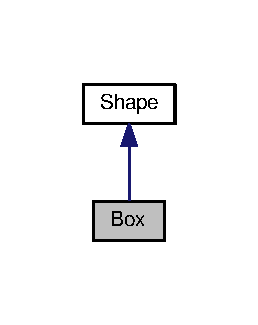
\includegraphics[width=124pt]{class_box__inherit__graph}
\end{center}
\end{figure}


Collaboration diagram for Box\+:
\nopagebreak
\begin{figure}[H]
\begin{center}
\leavevmode
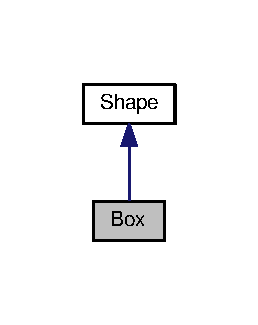
\includegraphics[width=124pt]{class_box__coll__graph}
\end{center}
\end{figure}
\subsection*{Public Member Functions}
\begin{DoxyCompactItemize}
\item 
\hyperlink{class_box_abfd946b41f47834eaa541b722bac9a29}{Box} (const glm\+::dvec3 \&box\+Min, const glm\+::dvec3 \&box\+Max, const glm\+::dvec4 \&color, const glm\+::dvec4 \&emissive, const glm\+::dvec4 \&reflect)
\item 
\hyperlink{class_shape}{Shape} $\ast$ \hyperlink{class_box_a4770c219ac36060feee72d02c45dab04}{copy} () const 
\item 
std\+::vector$<$ double $>$ \hyperlink{class_box_a32bbf5e25c16d002f2ff858177c25cd8}{intersect} (const \hyperlink{class_ray}{Ray} \&ray) const override
\item 
glm\+::dvec3 \hyperlink{class_box_a13821ada4849a78e238ced9260904a15}{normal} (const glm\+::dvec3 \&point) const override
\end{DoxyCompactItemize}


\subsection{Detailed Description}
Class representing a box in the scene. 

\subsection{Constructor \& Destructor Documentation}
\index{Box@{Box}!Box@{Box}}
\index{Box@{Box}!Box@{Box}}
\subsubsection[{\texorpdfstring{Box(const glm\+::dvec3 \&box\+Min, const glm\+::dvec3 \&box\+Max, const glm\+::dvec4 \&color, const glm\+::dvec4 \&emissive, const glm\+::dvec4 \&reflect)}{Box(const glm::dvec3 &boxMin, const glm::dvec3 &boxMax, const glm::dvec4 &color, const glm::dvec4 &emissive, const glm::dvec4 &reflect)}}]{\setlength{\rightskip}{0pt plus 5cm}Box\+::\+Box (
\begin{DoxyParamCaption}
\item[{const glm\+::dvec3 \&}]{box\+Min, }
\item[{const glm\+::dvec3 \&}]{box\+Max, }
\item[{const glm\+::dvec4 \&}]{color, }
\item[{const glm\+::dvec4 \&}]{emissive, }
\item[{const glm\+::dvec4 \&}]{reflect}
\end{DoxyParamCaption}
)\hspace{0.3cm}{\ttfamily [explicit]}}\hypertarget{class_box_abfd946b41f47834eaa541b722bac9a29}{}\label{class_box_abfd946b41f47834eaa541b722bac9a29}
Construct a box 
\begin{DoxyParams}{Parameters}
{\em box\+Min} & \+: Minimum point of the box \\
\hline
{\em box\+Max} & \+: Maximum point of the box \\
\hline
{\em color} & \+: Color of the box \\
\hline
{\em emissive} & \+: Emissive color of the box \\
\hline
{\em reflect} & \+: Reflection coefficients of the box \\
\hline
\end{DoxyParams}


\subsection{Member Function Documentation}
\index{Box@{Box}!copy@{copy}}
\index{copy@{copy}!Box@{Box}}
\subsubsection[{\texorpdfstring{copy() const }{copy() const }}]{\setlength{\rightskip}{0pt plus 5cm}{\bf Shape}$\ast$ Box\+::copy (
\begin{DoxyParamCaption}
{}
\end{DoxyParamCaption}
) const\hspace{0.3cm}{\ttfamily [virtual]}}\hypertarget{class_box_a4770c219ac36060feee72d02c45dab04}{}\label{class_box_a4770c219ac36060feee72d02c45dab04}
Copy the box \begin{DoxyReturn}{Returns}
a deep copy of the box 
\end{DoxyReturn}


Implements \hyperlink{class_shape_a99f9bc881b17366992a3edf278b105d0}{Shape}.

\index{Box@{Box}!intersect@{intersect}}
\index{intersect@{intersect}!Box@{Box}}
\subsubsection[{\texorpdfstring{intersect(const Ray \&ray) const override}{intersect(const Ray &ray) const override}}]{\setlength{\rightskip}{0pt plus 5cm}std\+::vector$<$double$>$ Box\+::intersect (
\begin{DoxyParamCaption}
\item[{const {\bf Ray} \&}]{ray}
\end{DoxyParamCaption}
) const\hspace{0.3cm}{\ttfamily [override]}, {\ttfamily [virtual]}}\hypertarget{class_box_a32bbf5e25c16d002f2ff858177c25cd8}{}\label{class_box_a32bbf5e25c16d002f2ff858177c25cd8}
Get the parametric values on the ray where the box is intersected

A point on a ray can be written as {\itshape O + tD}, where {\itshape O} is the origin, {\itshape D} the direction and {\itshape t} a scalar. This function will return all values {\itshape t} where the ray hit the box. If the ray did not hit the box, the returned vector is empty.


\begin{DoxyParams}{Parameters}
{\em ray} & Tested ray \\
\hline
\end{DoxyParams}
\begin{DoxyReturn}{Returns}
a vector containing all values {\itshape t} where the box is intersected 
\end{DoxyReturn}


Implements \hyperlink{class_shape_aa75a11aaba99bddfccf772faa7e6324b}{Shape}.

\index{Box@{Box}!normal@{normal}}
\index{normal@{normal}!Box@{Box}}
\subsubsection[{\texorpdfstring{normal(const glm\+::dvec3 \&point) const override}{normal(const glm::dvec3 &point) const override}}]{\setlength{\rightskip}{0pt plus 5cm}glm\+::dvec3 Box\+::normal (
\begin{DoxyParamCaption}
\item[{const glm\+::dvec3 \&}]{point}
\end{DoxyParamCaption}
) const\hspace{0.3cm}{\ttfamily [override]}, {\ttfamily [virtual]}}\hypertarget{class_box_a13821ada4849a78e238ced9260904a15}{}\label{class_box_a13821ada4849a78e238ced9260904a15}
Get the normal of the box at a particular point

The point have to be on the surface of the box.


\begin{DoxyParams}{Parameters}
{\em point} & Point where we want to retrieve the normal \\
\hline
\end{DoxyParams}
\begin{DoxyReturn}{Returns}
the normal of the box 
\end{DoxyReturn}


Implements \hyperlink{class_shape_a8444ffb396f26bd86c1c11bc6c47a74d}{Shape}.



The documentation for this class was generated from the following file\+:\begin{DoxyCompactItemize}
\item 
include/\hyperlink{box_8hpp}{box.\+hpp}\end{DoxyCompactItemize}

\hypertarget{class_camera}{}\section{Camera Class Reference}
\label{class_camera}\index{Camera@{Camera}}


Class representing a camera.  




{\ttfamily \#include $<$camera.\+hpp$>$}

\subsection*{Public Member Functions}
\begin{DoxyCompactItemize}
\item 
glm\+::dvec3 \hyperlink{class_camera_a8fd5bf11217034ce0f64e298f87dad60}{pixel\+Position} (int px, int py, double dz) const 
\item 
glm\+::dvec3 \hyperlink{class_camera_ae6d3cad7a69868bcc9ba1fd6a0350254}{get\+Position} () const 
\item 
int \hyperlink{class_camera_a220935f09adabbfa85511c799dbfb2b9}{get\+Screen\+Width} () const 
\item 
int \hyperlink{class_camera_a0448708fe31e35eb3f6413b1378143d8}{get\+Screen\+Height} () const 
\end{DoxyCompactItemize}
\subsection*{Static Public Member Functions}
\begin{DoxyCompactItemize}
\item 
static \hyperlink{class_camera}{Camera} \hyperlink{class_camera_ad396e8d09bbd305d055857806048ffc7}{create} (const glm\+::dvec3 \&position, const glm\+::dvec3 \&target, const glm\+::dvec3 \&up, double height\+Fov, int screen\+Width, int screen\+Height)
\end{DoxyCompactItemize}


\subsection{Detailed Description}
Class representing a camera. 

\subsection{Member Function Documentation}
\index{Camera@{Camera}!create@{create}}
\index{create@{create}!Camera@{Camera}}
\subsubsection[{\texorpdfstring{create(const glm\+::dvec3 \&position, const glm\+::dvec3 \&target, const glm\+::dvec3 \&up, double height\+Fov, int screen\+Width, int screen\+Height)}{create(const glm::dvec3 &position, const glm::dvec3 &target, const glm::dvec3 &up, double heightFov, int screenWidth, int screenHeight)}}]{\setlength{\rightskip}{0pt plus 5cm}static {\bf Camera} Camera\+::create (
\begin{DoxyParamCaption}
\item[{const glm\+::dvec3 \&}]{position, }
\item[{const glm\+::dvec3 \&}]{target, }
\item[{const glm\+::dvec3 \&}]{up, }
\item[{double}]{height\+Fov, }
\item[{int}]{screen\+Width, }
\item[{int}]{screen\+Height}
\end{DoxyParamCaption}
)\hspace{0.3cm}{\ttfamily [static]}}\hypertarget{class_camera_ad396e8d09bbd305d055857806048ffc7}{}\label{class_camera_ad396e8d09bbd305d055857806048ffc7}
Create a camera 
\begin{DoxyParams}{Parameters}
{\em position} & \+: Position of the camera \\
\hline
{\em target} & \+: Targeted point of the camera \\
\hline
{\em up} & \+: Up vector \\
\hline
{\em height\+Fov} & \+: Field of view angle in height \\
\hline
{\em screen\+Width} & \+: Width of the screen \\
\hline
{\em screen\+Height} & \+: Height of the screen \\
\hline
\end{DoxyParams}
\begin{DoxyReturn}{Returns}
the corresponding camera 
\end{DoxyReturn}
\index{Camera@{Camera}!get\+Position@{get\+Position}}
\index{get\+Position@{get\+Position}!Camera@{Camera}}
\subsubsection[{\texorpdfstring{get\+Position() const }{getPosition() const }}]{\setlength{\rightskip}{0pt plus 5cm}glm\+::dvec3 Camera\+::get\+Position (
\begin{DoxyParamCaption}
{}
\end{DoxyParamCaption}
) const}\hypertarget{class_camera_ae6d3cad7a69868bcc9ba1fd6a0350254}{}\label{class_camera_ae6d3cad7a69868bcc9ba1fd6a0350254}
Get the position of the camera \begin{DoxyReturn}{Returns}
the position of the camera 
\end{DoxyReturn}
\index{Camera@{Camera}!get\+Screen\+Height@{get\+Screen\+Height}}
\index{get\+Screen\+Height@{get\+Screen\+Height}!Camera@{Camera}}
\subsubsection[{\texorpdfstring{get\+Screen\+Height() const }{getScreenHeight() const }}]{\setlength{\rightskip}{0pt plus 5cm}int Camera\+::get\+Screen\+Height (
\begin{DoxyParamCaption}
{}
\end{DoxyParamCaption}
) const}\hypertarget{class_camera_a0448708fe31e35eb3f6413b1378143d8}{}\label{class_camera_a0448708fe31e35eb3f6413b1378143d8}
Get the height of the screen \begin{DoxyReturn}{Returns}
the height of the screen 
\end{DoxyReturn}
\index{Camera@{Camera}!get\+Screen\+Width@{get\+Screen\+Width}}
\index{get\+Screen\+Width@{get\+Screen\+Width}!Camera@{Camera}}
\subsubsection[{\texorpdfstring{get\+Screen\+Width() const }{getScreenWidth() const }}]{\setlength{\rightskip}{0pt plus 5cm}int Camera\+::get\+Screen\+Width (
\begin{DoxyParamCaption}
{}
\end{DoxyParamCaption}
) const}\hypertarget{class_camera_a220935f09adabbfa85511c799dbfb2b9}{}\label{class_camera_a220935f09adabbfa85511c799dbfb2b9}
Get the width of the screen \begin{DoxyReturn}{Returns}
the width of the screen 
\end{DoxyReturn}
\index{Camera@{Camera}!pixel\+Position@{pixel\+Position}}
\index{pixel\+Position@{pixel\+Position}!Camera@{Camera}}
\subsubsection[{\texorpdfstring{pixel\+Position(int px, int py, double dz) const }{pixelPosition(int px, int py, double dz) const }}]{\setlength{\rightskip}{0pt plus 5cm}glm\+::dvec3 Camera\+::pixel\+Position (
\begin{DoxyParamCaption}
\item[{int}]{px, }
\item[{int}]{py, }
\item[{double}]{dz}
\end{DoxyParamCaption}
) const}\hypertarget{class_camera_a8fd5bf11217034ce0f64e298f87dad60}{}\label{class_camera_a8fd5bf11217034ce0f64e298f87dad60}
Get the position of a pixel in the space 
\begin{DoxyParams}{Parameters}
{\em px} & \+: Coordinate value on the {\itshape x} axis of the pixel \\
\hline
{\em py} & \+: Coordinate value on the {\itshape y} axis of the pixel \\
\hline
{\em dz} & \+: Distance on the {\itshape z} axis \\
\hline
\end{DoxyParams}
\begin{DoxyReturn}{Returns}
the position of the pixel 
\end{DoxyReturn}


The documentation for this class was generated from the following file\+:\begin{DoxyCompactItemize}
\item 
include/\hyperlink{camera_8hpp}{camera.\+hpp}\end{DoxyCompactItemize}

\hypertarget{class_collision_point}{}\section{Collision\+Point Class Reference}
\label{class_collision_point}\index{Collision\+Point@{Collision\+Point}}


Class representing a collision point.  




{\ttfamily \#include $<$collision\+\_\+point.\+hpp$>$}

\subsection*{Public Member Functions}
\begin{DoxyCompactItemize}
\item 
\hyperlink{class_collision_point_ab5b42d7e054ed2d3bad382a30d7ac163}{Collision\+Point} (const glm\+::dvec3 \&point, const \hyperlink{class_shape}{Shape} $\ast$shape)
\item 
glm\+::dvec3 \hyperlink{class_collision_point_a81bc9e6bbde55ac5e39dc1454dc7cd5f}{get\+Point} () const 
\item 
const \hyperlink{class_shape}{Shape} $\ast$ \hyperlink{class_collision_point_a1b3a964945343a1f9d6ed69ee00f9497}{get\+Shape} () const 
\end{DoxyCompactItemize}


\subsection{Detailed Description}
Class representing a collision point. 

A collision point is represented by a point in the space and the shape to which it belongs. 

\subsection{Constructor \& Destructor Documentation}
\index{Collision\+Point@{Collision\+Point}!Collision\+Point@{Collision\+Point}}
\index{Collision\+Point@{Collision\+Point}!Collision\+Point@{Collision\+Point}}
\subsubsection[{\texorpdfstring{Collision\+Point(const glm\+::dvec3 \&point, const Shape $\ast$shape)}{CollisionPoint(const glm::dvec3 &point, const Shape *shape)}}]{\setlength{\rightskip}{0pt plus 5cm}Collision\+Point\+::\+Collision\+Point (
\begin{DoxyParamCaption}
\item[{const glm\+::dvec3 \&}]{point, }
\item[{const {\bf Shape} $\ast$}]{shape}
\end{DoxyParamCaption}
)\hspace{0.3cm}{\ttfamily [explicit]}}\hypertarget{class_collision_point_ab5b42d7e054ed2d3bad382a30d7ac163}{}\label{class_collision_point_ab5b42d7e054ed2d3bad382a30d7ac163}
Construct a collision point 
\begin{DoxyParams}{Parameters}
{\em point} & \+: Point of the collision \\
\hline
{\em shape} & \+: Collided shape \\
\hline
\end{DoxyParams}


\subsection{Member Function Documentation}
\index{Collision\+Point@{Collision\+Point}!get\+Point@{get\+Point}}
\index{get\+Point@{get\+Point}!Collision\+Point@{Collision\+Point}}
\subsubsection[{\texorpdfstring{get\+Point() const }{getPoint() const }}]{\setlength{\rightskip}{0pt plus 5cm}glm\+::dvec3 Collision\+Point\+::get\+Point (
\begin{DoxyParamCaption}
{}
\end{DoxyParamCaption}
) const}\hypertarget{class_collision_point_a81bc9e6bbde55ac5e39dc1454dc7cd5f}{}\label{class_collision_point_a81bc9e6bbde55ac5e39dc1454dc7cd5f}
Get the point of the collision \begin{DoxyReturn}{Returns}
the point of the collision 
\end{DoxyReturn}
\index{Collision\+Point@{Collision\+Point}!get\+Shape@{get\+Shape}}
\index{get\+Shape@{get\+Shape}!Collision\+Point@{Collision\+Point}}
\subsubsection[{\texorpdfstring{get\+Shape() const }{getShape() const }}]{\setlength{\rightskip}{0pt plus 5cm}const {\bf Shape}$\ast$ Collision\+Point\+::get\+Shape (
\begin{DoxyParamCaption}
{}
\end{DoxyParamCaption}
) const}\hypertarget{class_collision_point_a1b3a964945343a1f9d6ed69ee00f9497}{}\label{class_collision_point_a1b3a964945343a1f9d6ed69ee00f9497}
Get the collided shape \begin{DoxyReturn}{Returns}
the collided shape 
\end{DoxyReturn}


The documentation for this class was generated from the following file\+:\begin{DoxyCompactItemize}
\item 
include/collision\+\_\+point.\+hpp\end{DoxyCompactItemize}

\hypertarget{class_j_s_o_n_parser}{}\section{J\+S\+O\+N\+Parser Class Reference}
\label{class_j_s_o_n_parser}\index{J\+S\+O\+N\+Parser@{J\+S\+O\+N\+Parser}}


Helper class to parse the J\+S\+ON scene files.  




{\ttfamily \#include $<$json\+\_\+parser.\+hpp$>$}

\subsection*{Static Public Member Functions}
\begin{DoxyCompactItemize}
\item 
static std\+::pair$<$ \hyperlink{class_scene}{Scene}, \hyperlink{class_camera}{Camera} $>$ \hyperlink{class_j_s_o_n_parser_a0c127858348c36af0ac74a9653eaf6a0}{parse} (const std\+::string \&fname, int width, int height)
\end{DoxyCompactItemize}
\subsection*{Static Public Attributes}
\begin{DoxyCompactItemize}
\item 
static constexpr double \hyperlink{class_j_s_o_n_parser_a22e4a2b46ab4556ab6be042932ac60dc}{C\+A\+M\+E\+R\+A\+\_\+\+D\+E\+F\+A\+U\+L\+T\+\_\+\+H\+E\+I\+G\+H\+T\+\_\+\+F\+OV} = glm\+::pi$<$double$>$() / 5.\+0
\item 
static constexpr glm\+::dvec3 \hyperlink{class_j_s_o_n_parser_a2deb13759a25487b8033aaf84ac7c561}{C\+A\+M\+E\+R\+A\+\_\+\+D\+E\+F\+A\+U\+L\+T\+\_\+\+U\+P\+\_\+\+V\+E\+C\+T\+OR} = glm\+::dvec3(0.\+0, 1.\+0, 0.\+0)
\item 
static constexpr double \hyperlink{class_j_s_o_n_parser_a319445abcd1d1aebf5016488df6184ac}{S\+C\+E\+N\+E\+\_\+\+D\+E\+F\+A\+U\+L\+T\+\_\+\+D\+I\+S\+T\+A\+N\+C\+E\+\_\+\+N\+E\+AR} = 0.\+1
\item 
static constexpr double \hyperlink{class_j_s_o_n_parser_adcd06251c7b4b7ae8386d62dd4e72e07}{S\+C\+E\+N\+E\+\_\+\+D\+E\+F\+A\+U\+L\+T\+\_\+\+D\+I\+S\+T\+A\+N\+C\+E\+\_\+\+F\+AR} = 10000.\+0
\end{DoxyCompactItemize}


\subsection{Detailed Description}
Helper class to parse the J\+S\+ON scene files. 

\subsection{Member Function Documentation}
\index{J\+S\+O\+N\+Parser@{J\+S\+O\+N\+Parser}!parse@{parse}}
\index{parse@{parse}!J\+S\+O\+N\+Parser@{J\+S\+O\+N\+Parser}}
\subsubsection[{\texorpdfstring{parse(const std\+::string \&fname, int width, int height)}{parse(const std::string &fname, int width, int height)}}]{\setlength{\rightskip}{0pt plus 5cm}static std\+::pair$<${\bf Scene},{\bf Camera}$>$ J\+S\+O\+N\+Parser\+::parse (
\begin{DoxyParamCaption}
\item[{const std\+::string \&}]{fname, }
\item[{int}]{width, }
\item[{int}]{height}
\end{DoxyParamCaption}
)\hspace{0.3cm}{\ttfamily [static]}}\hypertarget{class_j_s_o_n_parser_a0c127858348c36af0ac74a9653eaf6a0}{}\label{class_j_s_o_n_parser_a0c127858348c36af0ac74a9653eaf6a0}
Parse a J\+S\+ON file scene

The description file contains the scene itself and the used camera to record the scene. Then the function return a pair of the scene and the camera described in the file. The camera is defined in the file by a position and a target. The scene is defined in the file by a list of shapes, a list of lights and a background color. For more precision on the format read the {\itshape R\+E\+A\+D\+M\+E.\+MD} file


\begin{DoxyParams}{Parameters}
{\em fname} & \+: File to parse \\
\hline
{\em width} & \+: Width of the image \\
\hline
{\em height} & \+: Height of the image \\
\hline
\end{DoxyParams}
\begin{DoxyReturn}{Returns}
the scene and the camera described in the file 
\end{DoxyReturn}


\subsection{Member Data Documentation}
\index{J\+S\+O\+N\+Parser@{J\+S\+O\+N\+Parser}!C\+A\+M\+E\+R\+A\+\_\+\+D\+E\+F\+A\+U\+L\+T\+\_\+\+H\+E\+I\+G\+H\+T\+\_\+\+F\+OV@{C\+A\+M\+E\+R\+A\+\_\+\+D\+E\+F\+A\+U\+L\+T\+\_\+\+H\+E\+I\+G\+H\+T\+\_\+\+F\+OV}}
\index{C\+A\+M\+E\+R\+A\+\_\+\+D\+E\+F\+A\+U\+L\+T\+\_\+\+H\+E\+I\+G\+H\+T\+\_\+\+F\+OV@{C\+A\+M\+E\+R\+A\+\_\+\+D\+E\+F\+A\+U\+L\+T\+\_\+\+H\+E\+I\+G\+H\+T\+\_\+\+F\+OV}!J\+S\+O\+N\+Parser@{J\+S\+O\+N\+Parser}}
\subsubsection[{\texorpdfstring{C\+A\+M\+E\+R\+A\+\_\+\+D\+E\+F\+A\+U\+L\+T\+\_\+\+H\+E\+I\+G\+H\+T\+\_\+\+F\+OV}{CAMERA_DEFAULT_HEIGHT_FOV}}]{\setlength{\rightskip}{0pt plus 5cm}constexpr double J\+S\+O\+N\+Parser\+::\+C\+A\+M\+E\+R\+A\+\_\+\+D\+E\+F\+A\+U\+L\+T\+\_\+\+H\+E\+I\+G\+H\+T\+\_\+\+F\+OV = glm\+::pi$<$double$>$() / 5.\+0\hspace{0.3cm}{\ttfamily [static]}}\hypertarget{class_j_s_o_n_parser_a22e4a2b46ab4556ab6be042932ac60dc}{}\label{class_j_s_o_n_parser_a22e4a2b46ab4556ab6be042932ac60dc}
Default value for the camera field of view angle in height \index{J\+S\+O\+N\+Parser@{J\+S\+O\+N\+Parser}!C\+A\+M\+E\+R\+A\+\_\+\+D\+E\+F\+A\+U\+L\+T\+\_\+\+U\+P\+\_\+\+V\+E\+C\+T\+OR@{C\+A\+M\+E\+R\+A\+\_\+\+D\+E\+F\+A\+U\+L\+T\+\_\+\+U\+P\+\_\+\+V\+E\+C\+T\+OR}}
\index{C\+A\+M\+E\+R\+A\+\_\+\+D\+E\+F\+A\+U\+L\+T\+\_\+\+U\+P\+\_\+\+V\+E\+C\+T\+OR@{C\+A\+M\+E\+R\+A\+\_\+\+D\+E\+F\+A\+U\+L\+T\+\_\+\+U\+P\+\_\+\+V\+E\+C\+T\+OR}!J\+S\+O\+N\+Parser@{J\+S\+O\+N\+Parser}}
\subsubsection[{\texorpdfstring{C\+A\+M\+E\+R\+A\+\_\+\+D\+E\+F\+A\+U\+L\+T\+\_\+\+U\+P\+\_\+\+V\+E\+C\+T\+OR}{CAMERA_DEFAULT_UP_VECTOR}}]{\setlength{\rightskip}{0pt plus 5cm}constexpr glm\+::dvec3 J\+S\+O\+N\+Parser\+::\+C\+A\+M\+E\+R\+A\+\_\+\+D\+E\+F\+A\+U\+L\+T\+\_\+\+U\+P\+\_\+\+V\+E\+C\+T\+OR = glm\+::dvec3(0.\+0, 1.\+0, 0.\+0)\hspace{0.3cm}{\ttfamily [static]}}\hypertarget{class_j_s_o_n_parser_a2deb13759a25487b8033aaf84ac7c561}{}\label{class_j_s_o_n_parser_a2deb13759a25487b8033aaf84ac7c561}
Default value for the camera up vector \index{J\+S\+O\+N\+Parser@{J\+S\+O\+N\+Parser}!S\+C\+E\+N\+E\+\_\+\+D\+E\+F\+A\+U\+L\+T\+\_\+\+D\+I\+S\+T\+A\+N\+C\+E\+\_\+\+F\+AR@{S\+C\+E\+N\+E\+\_\+\+D\+E\+F\+A\+U\+L\+T\+\_\+\+D\+I\+S\+T\+A\+N\+C\+E\+\_\+\+F\+AR}}
\index{S\+C\+E\+N\+E\+\_\+\+D\+E\+F\+A\+U\+L\+T\+\_\+\+D\+I\+S\+T\+A\+N\+C\+E\+\_\+\+F\+AR@{S\+C\+E\+N\+E\+\_\+\+D\+E\+F\+A\+U\+L\+T\+\_\+\+D\+I\+S\+T\+A\+N\+C\+E\+\_\+\+F\+AR}!J\+S\+O\+N\+Parser@{J\+S\+O\+N\+Parser}}
\subsubsection[{\texorpdfstring{S\+C\+E\+N\+E\+\_\+\+D\+E\+F\+A\+U\+L\+T\+\_\+\+D\+I\+S\+T\+A\+N\+C\+E\+\_\+\+F\+AR}{SCENE_DEFAULT_DISTANCE_FAR}}]{\setlength{\rightskip}{0pt plus 5cm}constexpr double J\+S\+O\+N\+Parser\+::\+S\+C\+E\+N\+E\+\_\+\+D\+E\+F\+A\+U\+L\+T\+\_\+\+D\+I\+S\+T\+A\+N\+C\+E\+\_\+\+F\+AR = 10000.\+0\hspace{0.3cm}{\ttfamily [static]}}\hypertarget{class_j_s_o_n_parser_adcd06251c7b4b7ae8386d62dd4e72e07}{}\label{class_j_s_o_n_parser_adcd06251c7b4b7ae8386d62dd4e72e07}
Default value for the scene maximum rendering distance \index{J\+S\+O\+N\+Parser@{J\+S\+O\+N\+Parser}!S\+C\+E\+N\+E\+\_\+\+D\+E\+F\+A\+U\+L\+T\+\_\+\+D\+I\+S\+T\+A\+N\+C\+E\+\_\+\+N\+E\+AR@{S\+C\+E\+N\+E\+\_\+\+D\+E\+F\+A\+U\+L\+T\+\_\+\+D\+I\+S\+T\+A\+N\+C\+E\+\_\+\+N\+E\+AR}}
\index{S\+C\+E\+N\+E\+\_\+\+D\+E\+F\+A\+U\+L\+T\+\_\+\+D\+I\+S\+T\+A\+N\+C\+E\+\_\+\+N\+E\+AR@{S\+C\+E\+N\+E\+\_\+\+D\+E\+F\+A\+U\+L\+T\+\_\+\+D\+I\+S\+T\+A\+N\+C\+E\+\_\+\+N\+E\+AR}!J\+S\+O\+N\+Parser@{J\+S\+O\+N\+Parser}}
\subsubsection[{\texorpdfstring{S\+C\+E\+N\+E\+\_\+\+D\+E\+F\+A\+U\+L\+T\+\_\+\+D\+I\+S\+T\+A\+N\+C\+E\+\_\+\+N\+E\+AR}{SCENE_DEFAULT_DISTANCE_NEAR}}]{\setlength{\rightskip}{0pt plus 5cm}constexpr double J\+S\+O\+N\+Parser\+::\+S\+C\+E\+N\+E\+\_\+\+D\+E\+F\+A\+U\+L\+T\+\_\+\+D\+I\+S\+T\+A\+N\+C\+E\+\_\+\+N\+E\+AR = 0.\+1\hspace{0.3cm}{\ttfamily [static]}}\hypertarget{class_j_s_o_n_parser_a319445abcd1d1aebf5016488df6184ac}{}\label{class_j_s_o_n_parser_a319445abcd1d1aebf5016488df6184ac}
Default value for the scene minimum rendering distance 

The documentation for this class was generated from the following file\+:\begin{DoxyCompactItemize}
\item 
include/\hyperlink{json__parser_8hpp}{json\+\_\+parser.\+hpp}\end{DoxyCompactItemize}

\hypertarget{class_light}{}\section{Light Class Reference}
\label{class_light}\index{Light@{Light}}


Class representing a light in the scene.  




{\ttfamily \#include $<$light.\+hpp$>$}

\subsection*{Public Member Functions}
\begin{DoxyCompactItemize}
\item 
\hyperlink{class_light_a9cf97d23d27489be4ab210f4340284e8}{Light} (const glm\+::dvec3 \&position, const glm\+::dvec4 \&color)
\item 
glm\+::dvec3 \hyperlink{class_light_a2161bd3f9f601ef59b15271cc6637340}{get\+Position} () const 
\item 
glm\+::dvec4 \hyperlink{class_light_afe910a49b79ab327e0d359c73d2db59d}{get\+Color} () const 
\end{DoxyCompactItemize}


\subsection{Detailed Description}
Class representing a light in the scene. 

\subsection{Constructor \& Destructor Documentation}
\index{Light@{Light}!Light@{Light}}
\index{Light@{Light}!Light@{Light}}
\subsubsection[{\texorpdfstring{Light(const glm\+::dvec3 \&position, const glm\+::dvec4 \&color)}{Light(const glm::dvec3 &position, const glm::dvec4 &color)}}]{\setlength{\rightskip}{0pt plus 5cm}Light\+::\+Light (
\begin{DoxyParamCaption}
\item[{const glm\+::dvec3 \&}]{position, }
\item[{const glm\+::dvec4 \&}]{color}
\end{DoxyParamCaption}
)\hspace{0.3cm}{\ttfamily [explicit]}}\hypertarget{class_light_a9cf97d23d27489be4ab210f4340284e8}{}\label{class_light_a9cf97d23d27489be4ab210f4340284e8}
Construct a light 
\begin{DoxyParams}{Parameters}
{\em position} & \+: Position of the light \\
\hline
{\em color} & \+: Color of the light \\
\hline
\end{DoxyParams}


\subsection{Member Function Documentation}
\index{Light@{Light}!get\+Color@{get\+Color}}
\index{get\+Color@{get\+Color}!Light@{Light}}
\subsubsection[{\texorpdfstring{get\+Color() const }{getColor() const }}]{\setlength{\rightskip}{0pt plus 5cm}glm\+::dvec4 Light\+::get\+Color (
\begin{DoxyParamCaption}
{}
\end{DoxyParamCaption}
) const}\hypertarget{class_light_afe910a49b79ab327e0d359c73d2db59d}{}\label{class_light_afe910a49b79ab327e0d359c73d2db59d}
Get the color of the light \begin{DoxyReturn}{Returns}
the color of the light 
\end{DoxyReturn}
\index{Light@{Light}!get\+Position@{get\+Position}}
\index{get\+Position@{get\+Position}!Light@{Light}}
\subsubsection[{\texorpdfstring{get\+Position() const }{getPosition() const }}]{\setlength{\rightskip}{0pt plus 5cm}glm\+::dvec3 Light\+::get\+Position (
\begin{DoxyParamCaption}
{}
\end{DoxyParamCaption}
) const}\hypertarget{class_light_a2161bd3f9f601ef59b15271cc6637340}{}\label{class_light_a2161bd3f9f601ef59b15271cc6637340}
Get the position of the light \begin{DoxyReturn}{Returns}
the position of the light 
\end{DoxyReturn}


The documentation for this class was generated from the following file\+:\begin{DoxyCompactItemize}
\item 
include/\hyperlink{light_8hpp}{light.\+hpp}\end{DoxyCompactItemize}

\hypertarget{struct_lode_p_n_g_color_mode}{}\section{Lode\+P\+N\+G\+Color\+Mode Struct Reference}
\label{struct_lode_p_n_g_color_mode}\index{Lode\+P\+N\+G\+Color\+Mode@{Lode\+P\+N\+G\+Color\+Mode}}
\subsection*{Public Attributes}
\begin{DoxyCompactItemize}
\item 
Lode\+P\+N\+G\+Color\+Type {\bfseries colortype}\hypertarget{struct_lode_p_n_g_color_mode_a4f3df7240411abe80546052d197fbe8d}{}\label{struct_lode_p_n_g_color_mode_a4f3df7240411abe80546052d197fbe8d}

\item 
unsigned {\bfseries bitdepth}\hypertarget{struct_lode_p_n_g_color_mode_ad20010b9561980f65281bc17f7848253}{}\label{struct_lode_p_n_g_color_mode_ad20010b9561980f65281bc17f7848253}

\item 
unsigned char $\ast$ {\bfseries palette}\hypertarget{struct_lode_p_n_g_color_mode_a54f0a793238009fcb95f081626fae308}{}\label{struct_lode_p_n_g_color_mode_a54f0a793238009fcb95f081626fae308}

\item 
size\+\_\+t {\bfseries palettesize}\hypertarget{struct_lode_p_n_g_color_mode_a407557f056168682d9319aeb60866dcc}{}\label{struct_lode_p_n_g_color_mode_a407557f056168682d9319aeb60866dcc}

\item 
unsigned {\bfseries key\+\_\+defined}\hypertarget{struct_lode_p_n_g_color_mode_ab9105505c5d56cfc6ce4efe1bb288b54}{}\label{struct_lode_p_n_g_color_mode_ab9105505c5d56cfc6ce4efe1bb288b54}

\item 
unsigned {\bfseries key\+\_\+r}\hypertarget{struct_lode_p_n_g_color_mode_a29e64327bca1f3d16235e9ff471e4d50}{}\label{struct_lode_p_n_g_color_mode_a29e64327bca1f3d16235e9ff471e4d50}

\item 
unsigned {\bfseries key\+\_\+g}\hypertarget{struct_lode_p_n_g_color_mode_ad98309f36d289392b0c440baa50af9f6}{}\label{struct_lode_p_n_g_color_mode_ad98309f36d289392b0c440baa50af9f6}

\item 
unsigned {\bfseries key\+\_\+b}\hypertarget{struct_lode_p_n_g_color_mode_a93a269405fee0d1c5045a1a671ed1de8}{}\label{struct_lode_p_n_g_color_mode_a93a269405fee0d1c5045a1a671ed1de8}

\end{DoxyCompactItemize}


The documentation for this struct was generated from the following file\+:\begin{DoxyCompactItemize}
\item 
include/lodepng.\+h\end{DoxyCompactItemize}

\hypertarget{struct_lode_p_n_g_color_profile}{}\section{Lode\+P\+N\+G\+Color\+Profile Struct Reference}
\label{struct_lode_p_n_g_color_profile}\index{Lode\+P\+N\+G\+Color\+Profile@{Lode\+P\+N\+G\+Color\+Profile}}
\subsection*{Public Attributes}
\begin{DoxyCompactItemize}
\item 
unsigned {\bfseries colored}\hypertarget{struct_lode_p_n_g_color_profile_abf063a566a4ab9f4d71b49764573d610}{}\label{struct_lode_p_n_g_color_profile_abf063a566a4ab9f4d71b49764573d610}

\item 
unsigned {\bfseries key}\hypertarget{struct_lode_p_n_g_color_profile_a24f19f400a53672340877eefbc837b0c}{}\label{struct_lode_p_n_g_color_profile_a24f19f400a53672340877eefbc837b0c}

\item 
unsigned short {\bfseries key\+\_\+r}\hypertarget{struct_lode_p_n_g_color_profile_a0398985ae0572ef97e83c33c7486cafd}{}\label{struct_lode_p_n_g_color_profile_a0398985ae0572ef97e83c33c7486cafd}

\item 
unsigned short {\bfseries key\+\_\+g}\hypertarget{struct_lode_p_n_g_color_profile_aba03e973374bd15315b8c01b86e94e8f}{}\label{struct_lode_p_n_g_color_profile_aba03e973374bd15315b8c01b86e94e8f}

\item 
unsigned short {\bfseries key\+\_\+b}\hypertarget{struct_lode_p_n_g_color_profile_a39b65ec69f6aaee3ee7312a993f21e40}{}\label{struct_lode_p_n_g_color_profile_a39b65ec69f6aaee3ee7312a993f21e40}

\item 
unsigned {\bfseries alpha}\hypertarget{struct_lode_p_n_g_color_profile_a554fea329af8034e91e1cdd8c1af0d90}{}\label{struct_lode_p_n_g_color_profile_a554fea329af8034e91e1cdd8c1af0d90}

\item 
unsigned {\bfseries numcolors}\hypertarget{struct_lode_p_n_g_color_profile_afdce0f5fbec46d6b8f1ec63da0a285f9}{}\label{struct_lode_p_n_g_color_profile_afdce0f5fbec46d6b8f1ec63da0a285f9}

\item 
unsigned char {\bfseries palette} \mbox{[}1024\mbox{]}\hypertarget{struct_lode_p_n_g_color_profile_a223f8bee4c9ae8be0b70cc08f19aaead}{}\label{struct_lode_p_n_g_color_profile_a223f8bee4c9ae8be0b70cc08f19aaead}

\item 
unsigned {\bfseries bits}\hypertarget{struct_lode_p_n_g_color_profile_a1d3870b03dfe6d699bf4c968c9bc1890}{}\label{struct_lode_p_n_g_color_profile_a1d3870b03dfe6d699bf4c968c9bc1890}

\end{DoxyCompactItemize}


The documentation for this struct was generated from the following file\+:\begin{DoxyCompactItemize}
\item 
include/lodepng.\+h\end{DoxyCompactItemize}

\hypertarget{struct_lode_p_n_g_compress_settings}{}\section{Lode\+P\+N\+G\+Compress\+Settings Struct Reference}
\label{struct_lode_p_n_g_compress_settings}\index{Lode\+P\+N\+G\+Compress\+Settings@{Lode\+P\+N\+G\+Compress\+Settings}}
\subsection*{Public Attributes}
\begin{DoxyCompactItemize}
\item 
unsigned {\bfseries btype}\hypertarget{struct_lode_p_n_g_compress_settings_ac0afeac7276cce01fa9824aa2d5a1ba9}{}\label{struct_lode_p_n_g_compress_settings_ac0afeac7276cce01fa9824aa2d5a1ba9}

\item 
unsigned {\bfseries use\+\_\+lz77}\hypertarget{struct_lode_p_n_g_compress_settings_a37a87bd874376f0298efad2870e70e7e}{}\label{struct_lode_p_n_g_compress_settings_a37a87bd874376f0298efad2870e70e7e}

\item 
unsigned {\bfseries windowsize}\hypertarget{struct_lode_p_n_g_compress_settings_a01e77a9db5c2c4dfe6c79bf04f0bf84e}{}\label{struct_lode_p_n_g_compress_settings_a01e77a9db5c2c4dfe6c79bf04f0bf84e}

\item 
unsigned {\bfseries minmatch}\hypertarget{struct_lode_p_n_g_compress_settings_a11d89e0ff0c57f1c49dd58cb8347e005}{}\label{struct_lode_p_n_g_compress_settings_a11d89e0ff0c57f1c49dd58cb8347e005}

\item 
unsigned {\bfseries nicematch}\hypertarget{struct_lode_p_n_g_compress_settings_a70bc37e21eeffead6e9c8d67e163a591}{}\label{struct_lode_p_n_g_compress_settings_a70bc37e21eeffead6e9c8d67e163a591}

\item 
unsigned {\bfseries lazymatching}\hypertarget{struct_lode_p_n_g_compress_settings_ad4ffde429dee40a8c314016f5f6fdab5}{}\label{struct_lode_p_n_g_compress_settings_ad4ffde429dee40a8c314016f5f6fdab5}

\item 
unsigned($\ast$ {\bfseries custom\+\_\+zlib} )(unsigned char $\ast$$\ast$, size\+\_\+t $\ast$, const unsigned char $\ast$, size\+\_\+t, const \hyperlink{struct_lode_p_n_g_compress_settings}{Lode\+P\+N\+G\+Compress\+Settings} $\ast$)\hypertarget{struct_lode_p_n_g_compress_settings_a4a7835f394349f15f1302d11bcb0efa0}{}\label{struct_lode_p_n_g_compress_settings_a4a7835f394349f15f1302d11bcb0efa0}

\item 
unsigned($\ast$ {\bfseries custom\+\_\+deflate} )(unsigned char $\ast$$\ast$, size\+\_\+t $\ast$, const unsigned char $\ast$, size\+\_\+t, const \hyperlink{struct_lode_p_n_g_compress_settings}{Lode\+P\+N\+G\+Compress\+Settings} $\ast$)\hypertarget{struct_lode_p_n_g_compress_settings_a55dafebbbe017806fb2bbc32bb40a59b}{}\label{struct_lode_p_n_g_compress_settings_a55dafebbbe017806fb2bbc32bb40a59b}

\item 
const void $\ast$ {\bfseries custom\+\_\+context}\hypertarget{struct_lode_p_n_g_compress_settings_a62826645ef28e2a84dd2b65f547a2883}{}\label{struct_lode_p_n_g_compress_settings_a62826645ef28e2a84dd2b65f547a2883}

\end{DoxyCompactItemize}


The documentation for this struct was generated from the following file\+:\begin{DoxyCompactItemize}
\item 
include/lodepng.\+h\end{DoxyCompactItemize}

\hypertarget{struct_lode_p_n_g_decoder_settings}{}\section{Lode\+P\+N\+G\+Decoder\+Settings Struct Reference}
\label{struct_lode_p_n_g_decoder_settings}\index{Lode\+P\+N\+G\+Decoder\+Settings@{Lode\+P\+N\+G\+Decoder\+Settings}}


Collaboration diagram for Lode\+P\+N\+G\+Decoder\+Settings\+:
\nopagebreak
\begin{figure}[H]
\begin{center}
\leavevmode
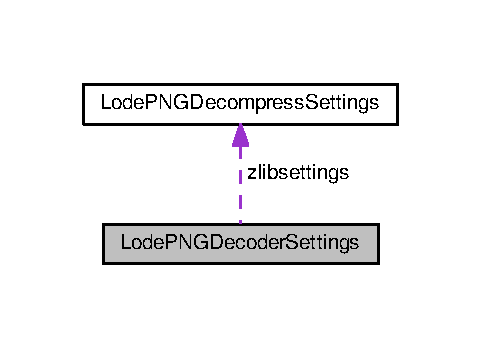
\includegraphics[width=231pt]{struct_lode_p_n_g_decoder_settings__coll__graph}
\end{center}
\end{figure}
\subsection*{Public Attributes}
\begin{DoxyCompactItemize}
\item 
\hyperlink{struct_lode_p_n_g_decompress_settings}{Lode\+P\+N\+G\+Decompress\+Settings} {\bfseries zlibsettings}\hypertarget{struct_lode_p_n_g_decoder_settings_a9ae8fef9880bef97a3e932f8ea942ed8}{}\label{struct_lode_p_n_g_decoder_settings_a9ae8fef9880bef97a3e932f8ea942ed8}

\item 
unsigned {\bfseries ignore\+\_\+crc}\hypertarget{struct_lode_p_n_g_decoder_settings_a6390c403d2a5718242337bbbaf15131d}{}\label{struct_lode_p_n_g_decoder_settings_a6390c403d2a5718242337bbbaf15131d}

\item 
unsigned {\bfseries ignore\+\_\+critical}\hypertarget{struct_lode_p_n_g_decoder_settings_a51c3ce791f1b1d325d5e1f7e18caeeea}{}\label{struct_lode_p_n_g_decoder_settings_a51c3ce791f1b1d325d5e1f7e18caeeea}

\item 
unsigned {\bfseries ignore\+\_\+end}\hypertarget{struct_lode_p_n_g_decoder_settings_aa8f3907b3dcaf09892a752806be2fc59}{}\label{struct_lode_p_n_g_decoder_settings_aa8f3907b3dcaf09892a752806be2fc59}

\item 
unsigned {\bfseries color\+\_\+convert}\hypertarget{struct_lode_p_n_g_decoder_settings_af26f2b29cd338ce4476bee9571a0818a}{}\label{struct_lode_p_n_g_decoder_settings_af26f2b29cd338ce4476bee9571a0818a}

\item 
unsigned {\bfseries read\+\_\+text\+\_\+chunks}\hypertarget{struct_lode_p_n_g_decoder_settings_aa1212905c3f73d9fffef2c04a220d951}{}\label{struct_lode_p_n_g_decoder_settings_aa1212905c3f73d9fffef2c04a220d951}

\item 
unsigned {\bfseries remember\+\_\+unknown\+\_\+chunks}\hypertarget{struct_lode_p_n_g_decoder_settings_a8775e4fc539dc457916720f52b442f27}{}\label{struct_lode_p_n_g_decoder_settings_a8775e4fc539dc457916720f52b442f27}

\end{DoxyCompactItemize}


The documentation for this struct was generated from the following file\+:\begin{DoxyCompactItemize}
\item 
include/lodepng.\+h\end{DoxyCompactItemize}

\hypertarget{struct_lode_p_n_g_decompress_settings}{}\section{Lode\+P\+N\+G\+Decompress\+Settings Struct Reference}
\label{struct_lode_p_n_g_decompress_settings}\index{Lode\+P\+N\+G\+Decompress\+Settings@{Lode\+P\+N\+G\+Decompress\+Settings}}
\subsection*{Public Attributes}
\begin{DoxyCompactItemize}
\item 
unsigned {\bfseries ignore\+\_\+adler32}\hypertarget{struct_lode_p_n_g_decompress_settings_afab4b919650b51b4d2f175a60ed6c580}{}\label{struct_lode_p_n_g_decompress_settings_afab4b919650b51b4d2f175a60ed6c580}

\item 
unsigned($\ast$ {\bfseries custom\+\_\+zlib} )(unsigned char $\ast$$\ast$, size\+\_\+t $\ast$, const unsigned char $\ast$, size\+\_\+t, const \hyperlink{struct_lode_p_n_g_decompress_settings}{Lode\+P\+N\+G\+Decompress\+Settings} $\ast$)\hypertarget{struct_lode_p_n_g_decompress_settings_a9dd432e46330dbd2ce3ef1929c64337d}{}\label{struct_lode_p_n_g_decompress_settings_a9dd432e46330dbd2ce3ef1929c64337d}

\item 
unsigned($\ast$ {\bfseries custom\+\_\+inflate} )(unsigned char $\ast$$\ast$, size\+\_\+t $\ast$, const unsigned char $\ast$, size\+\_\+t, const \hyperlink{struct_lode_p_n_g_decompress_settings}{Lode\+P\+N\+G\+Decompress\+Settings} $\ast$)\hypertarget{struct_lode_p_n_g_decompress_settings_a023aa5946c99934d40280850a4d8b204}{}\label{struct_lode_p_n_g_decompress_settings_a023aa5946c99934d40280850a4d8b204}

\item 
const void $\ast$ {\bfseries custom\+\_\+context}\hypertarget{struct_lode_p_n_g_decompress_settings_a66e3608b541c64bb275c0ac1a80c3ec6}{}\label{struct_lode_p_n_g_decompress_settings_a66e3608b541c64bb275c0ac1a80c3ec6}

\end{DoxyCompactItemize}


The documentation for this struct was generated from the following file\+:\begin{DoxyCompactItemize}
\item 
include/lodepng.\+h\end{DoxyCompactItemize}

\hypertarget{struct_lode_p_n_g_encoder_settings}{}\section{Lode\+P\+N\+G\+Encoder\+Settings Struct Reference}
\label{struct_lode_p_n_g_encoder_settings}\index{Lode\+P\+N\+G\+Encoder\+Settings@{Lode\+P\+N\+G\+Encoder\+Settings}}


Collaboration diagram for Lode\+P\+N\+G\+Encoder\+Settings\+:
\nopagebreak
\begin{figure}[H]
\begin{center}
\leavevmode
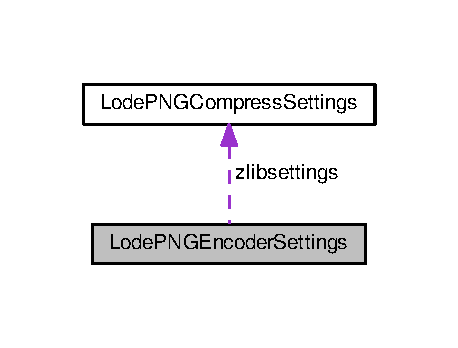
\includegraphics[width=220pt]{struct_lode_p_n_g_encoder_settings__coll__graph}
\end{center}
\end{figure}
\subsection*{Public Attributes}
\begin{DoxyCompactItemize}
\item 
\hyperlink{struct_lode_p_n_g_compress_settings}{Lode\+P\+N\+G\+Compress\+Settings} {\bfseries zlibsettings}\hypertarget{struct_lode_p_n_g_encoder_settings_a2c5928b4172c75e27de467870f2ff946}{}\label{struct_lode_p_n_g_encoder_settings_a2c5928b4172c75e27de467870f2ff946}

\item 
unsigned {\bfseries auto\+\_\+convert}\hypertarget{struct_lode_p_n_g_encoder_settings_a1203b8db6532c9ff4a5c8ee692cd327a}{}\label{struct_lode_p_n_g_encoder_settings_a1203b8db6532c9ff4a5c8ee692cd327a}

\item 
unsigned {\bfseries filter\+\_\+palette\+\_\+zero}\hypertarget{struct_lode_p_n_g_encoder_settings_a0d82e8f2fabcb6cebbc54b80922945f1}{}\label{struct_lode_p_n_g_encoder_settings_a0d82e8f2fabcb6cebbc54b80922945f1}

\item 
Lode\+P\+N\+G\+Filter\+Strategy {\bfseries filter\+\_\+strategy}\hypertarget{struct_lode_p_n_g_encoder_settings_a5e18e4eb941763a2e3e6c65ee9f0729c}{}\label{struct_lode_p_n_g_encoder_settings_a5e18e4eb941763a2e3e6c65ee9f0729c}

\item 
const unsigned char $\ast$ {\bfseries predefined\+\_\+filters}\hypertarget{struct_lode_p_n_g_encoder_settings_a4446f87b5283f25664802a1be037e76e}{}\label{struct_lode_p_n_g_encoder_settings_a4446f87b5283f25664802a1be037e76e}

\item 
unsigned {\bfseries force\+\_\+palette}\hypertarget{struct_lode_p_n_g_encoder_settings_a04dc9622ccd1d7c74c56291409aa512a}{}\label{struct_lode_p_n_g_encoder_settings_a04dc9622ccd1d7c74c56291409aa512a}

\item 
unsigned {\bfseries add\+\_\+id}\hypertarget{struct_lode_p_n_g_encoder_settings_a893aa542aa7c122c32ee36dd716fbcb2}{}\label{struct_lode_p_n_g_encoder_settings_a893aa542aa7c122c32ee36dd716fbcb2}

\item 
unsigned {\bfseries text\+\_\+compression}\hypertarget{struct_lode_p_n_g_encoder_settings_a6ffdcb8e85a65ea208fe027be072d710}{}\label{struct_lode_p_n_g_encoder_settings_a6ffdcb8e85a65ea208fe027be072d710}

\end{DoxyCompactItemize}


The documentation for this struct was generated from the following file\+:\begin{DoxyCompactItemize}
\item 
include/lodepng.\+h\end{DoxyCompactItemize}

\hypertarget{struct_lode_p_n_g_info}{}\section{Lode\+P\+N\+G\+Info Struct Reference}
\label{struct_lode_p_n_g_info}\index{Lode\+P\+N\+G\+Info@{Lode\+P\+N\+G\+Info}}


Collaboration diagram for Lode\+P\+N\+G\+Info\+:
\nopagebreak
\begin{figure}[H]
\begin{center}
\leavevmode
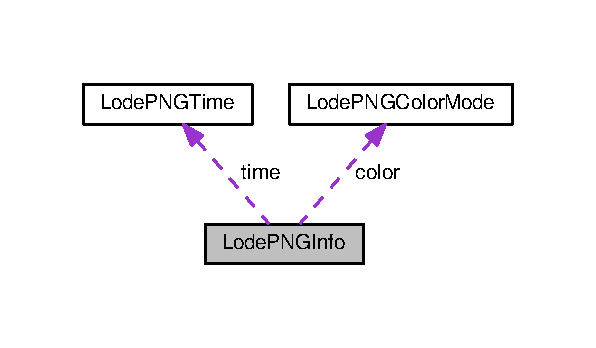
\includegraphics[width=286pt]{struct_lode_p_n_g_info__coll__graph}
\end{center}
\end{figure}
\subsection*{Public Attributes}
\begin{DoxyCompactItemize}
\item 
unsigned {\bfseries compression\+\_\+method}\hypertarget{struct_lode_p_n_g_info_a42bcacd0dbaaea01c04cc87b58ac3c1d}{}\label{struct_lode_p_n_g_info_a42bcacd0dbaaea01c04cc87b58ac3c1d}

\item 
unsigned {\bfseries filter\+\_\+method}\hypertarget{struct_lode_p_n_g_info_a5098d6e8aa528d5197f51914439633b9}{}\label{struct_lode_p_n_g_info_a5098d6e8aa528d5197f51914439633b9}

\item 
unsigned {\bfseries interlace\+\_\+method}\hypertarget{struct_lode_p_n_g_info_a80207e3e53c959b2285636496a3dd3f1}{}\label{struct_lode_p_n_g_info_a80207e3e53c959b2285636496a3dd3f1}

\item 
\hyperlink{struct_lode_p_n_g_color_mode}{Lode\+P\+N\+G\+Color\+Mode} {\bfseries color}\hypertarget{struct_lode_p_n_g_info_a0af9bab3435084780ce8c1cb69bb2628}{}\label{struct_lode_p_n_g_info_a0af9bab3435084780ce8c1cb69bb2628}

\item 
unsigned {\bfseries background\+\_\+defined}\hypertarget{struct_lode_p_n_g_info_aa94c65344af02472adb9c71eae2e765f}{}\label{struct_lode_p_n_g_info_aa94c65344af02472adb9c71eae2e765f}

\item 
unsigned {\bfseries background\+\_\+r}\hypertarget{struct_lode_p_n_g_info_a98b59c3760bda184bb16c9713b430bc3}{}\label{struct_lode_p_n_g_info_a98b59c3760bda184bb16c9713b430bc3}

\item 
unsigned {\bfseries background\+\_\+g}\hypertarget{struct_lode_p_n_g_info_abf638e191edaeaa2b02c371a381e3a89}{}\label{struct_lode_p_n_g_info_abf638e191edaeaa2b02c371a381e3a89}

\item 
unsigned {\bfseries background\+\_\+b}\hypertarget{struct_lode_p_n_g_info_a994de0c74ef1092f056ff534e00dfa0d}{}\label{struct_lode_p_n_g_info_a994de0c74ef1092f056ff534e00dfa0d}

\item 
size\+\_\+t {\bfseries text\+\_\+num}\hypertarget{struct_lode_p_n_g_info_a393e0b3948ca6674232e1cc625db282e}{}\label{struct_lode_p_n_g_info_a393e0b3948ca6674232e1cc625db282e}

\item 
char $\ast$$\ast$ {\bfseries text\+\_\+keys}\hypertarget{struct_lode_p_n_g_info_a0a26147c9673870dd122693f17a69b13}{}\label{struct_lode_p_n_g_info_a0a26147c9673870dd122693f17a69b13}

\item 
char $\ast$$\ast$ {\bfseries text\+\_\+strings}\hypertarget{struct_lode_p_n_g_info_aac321d27e65c54e56d6092d3a6400a81}{}\label{struct_lode_p_n_g_info_aac321d27e65c54e56d6092d3a6400a81}

\item 
size\+\_\+t {\bfseries itext\+\_\+num}\hypertarget{struct_lode_p_n_g_info_a22166bb10c89a4d80e206d6c4736b625}{}\label{struct_lode_p_n_g_info_a22166bb10c89a4d80e206d6c4736b625}

\item 
char $\ast$$\ast$ {\bfseries itext\+\_\+keys}\hypertarget{struct_lode_p_n_g_info_a1b909e03596abf86d564641741b0087f}{}\label{struct_lode_p_n_g_info_a1b909e03596abf86d564641741b0087f}

\item 
char $\ast$$\ast$ {\bfseries itext\+\_\+langtags}\hypertarget{struct_lode_p_n_g_info_ae9f9f594e63c910d467a14f550960837}{}\label{struct_lode_p_n_g_info_ae9f9f594e63c910d467a14f550960837}

\item 
char $\ast$$\ast$ {\bfseries itext\+\_\+transkeys}\hypertarget{struct_lode_p_n_g_info_a93a8e823ac715dbdd625f023d8fdebc2}{}\label{struct_lode_p_n_g_info_a93a8e823ac715dbdd625f023d8fdebc2}

\item 
char $\ast$$\ast$ {\bfseries itext\+\_\+strings}\hypertarget{struct_lode_p_n_g_info_a7014fd40ffeb1d482f72d33c020cf73e}{}\label{struct_lode_p_n_g_info_a7014fd40ffeb1d482f72d33c020cf73e}

\item 
unsigned {\bfseries time\+\_\+defined}\hypertarget{struct_lode_p_n_g_info_a9adb9f74ab90716ae107b99da5384424}{}\label{struct_lode_p_n_g_info_a9adb9f74ab90716ae107b99da5384424}

\item 
\hyperlink{struct_lode_p_n_g_time}{Lode\+P\+N\+G\+Time} {\bfseries time}\hypertarget{struct_lode_p_n_g_info_a4d3407acdf79bf87f20a3562f210b393}{}\label{struct_lode_p_n_g_info_a4d3407acdf79bf87f20a3562f210b393}

\item 
unsigned {\bfseries phys\+\_\+defined}\hypertarget{struct_lode_p_n_g_info_a9b8e29b7e7b4908a2de0275e01a828ed}{}\label{struct_lode_p_n_g_info_a9b8e29b7e7b4908a2de0275e01a828ed}

\item 
unsigned {\bfseries phys\+\_\+x}\hypertarget{struct_lode_p_n_g_info_a1593fa6e1acc93f3b9de51c340bef94d}{}\label{struct_lode_p_n_g_info_a1593fa6e1acc93f3b9de51c340bef94d}

\item 
unsigned {\bfseries phys\+\_\+y}\hypertarget{struct_lode_p_n_g_info_a52ad7a105244d00f1e91c489eaf53f97}{}\label{struct_lode_p_n_g_info_a52ad7a105244d00f1e91c489eaf53f97}

\item 
unsigned {\bfseries phys\+\_\+unit}\hypertarget{struct_lode_p_n_g_info_ad6f2171d9f87716e5010f6c5352f9855}{}\label{struct_lode_p_n_g_info_ad6f2171d9f87716e5010f6c5352f9855}

\item 
unsigned char $\ast$ {\bfseries unknown\+\_\+chunks\+\_\+data} \mbox{[}3\mbox{]}\hypertarget{struct_lode_p_n_g_info_a8347476da7fc2fc6af4ec7ed44b638c6}{}\label{struct_lode_p_n_g_info_a8347476da7fc2fc6af4ec7ed44b638c6}

\item 
size\+\_\+t {\bfseries unknown\+\_\+chunks\+\_\+size} \mbox{[}3\mbox{]}\hypertarget{struct_lode_p_n_g_info_a25a81d760759bd0383ae5a81ba83911d}{}\label{struct_lode_p_n_g_info_a25a81d760759bd0383ae5a81ba83911d}

\end{DoxyCompactItemize}


The documentation for this struct was generated from the following file\+:\begin{DoxyCompactItemize}
\item 
include/lodepng.\+h\end{DoxyCompactItemize}

\hypertarget{struct_lode_p_n_g_state}{}\section{Lode\+P\+N\+G\+State Struct Reference}
\label{struct_lode_p_n_g_state}\index{Lode\+P\+N\+G\+State@{Lode\+P\+N\+G\+State}}


Collaboration diagram for Lode\+P\+N\+G\+State\+:
\nopagebreak
\begin{figure}[H]
\begin{center}
\leavevmode
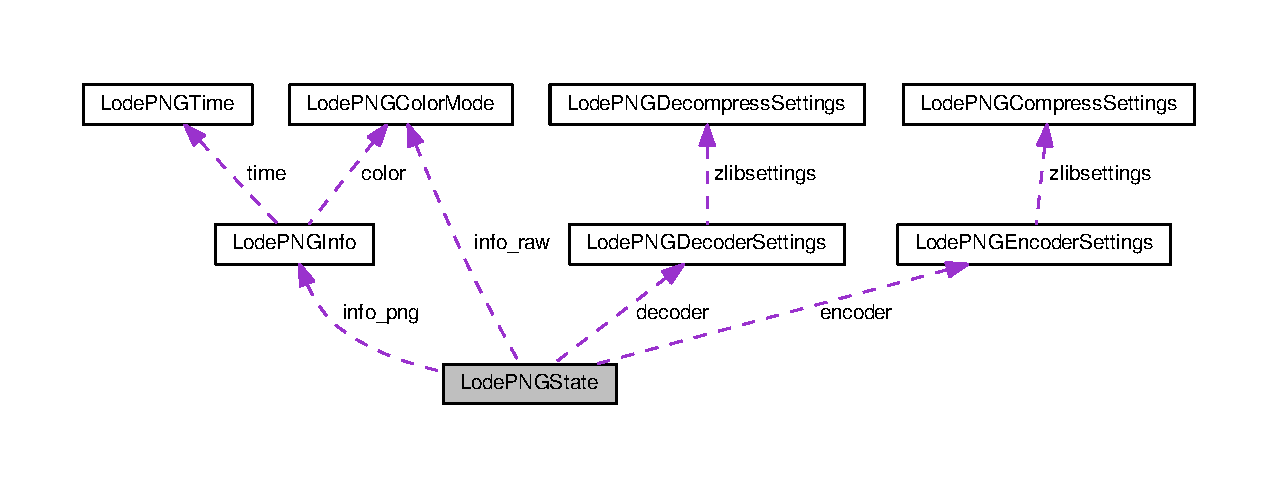
\includegraphics[width=350pt]{struct_lode_p_n_g_state__coll__graph}
\end{center}
\end{figure}
\subsection*{Public Attributes}
\begin{DoxyCompactItemize}
\item 
\hyperlink{struct_lode_p_n_g_decoder_settings}{Lode\+P\+N\+G\+Decoder\+Settings} {\bfseries decoder}\hypertarget{struct_lode_p_n_g_state_abd2c38ffc68f04b0e4159e1f97ba1f76}{}\label{struct_lode_p_n_g_state_abd2c38ffc68f04b0e4159e1f97ba1f76}

\item 
\hyperlink{struct_lode_p_n_g_encoder_settings}{Lode\+P\+N\+G\+Encoder\+Settings} {\bfseries encoder}\hypertarget{struct_lode_p_n_g_state_ac63d91db835129d02eb83bbe81de347e}{}\label{struct_lode_p_n_g_state_ac63d91db835129d02eb83bbe81de347e}

\item 
\hyperlink{struct_lode_p_n_g_color_mode}{Lode\+P\+N\+G\+Color\+Mode} {\bfseries info\+\_\+raw}\hypertarget{struct_lode_p_n_g_state_a597bc08de787147474d43adf8b6ceacf}{}\label{struct_lode_p_n_g_state_a597bc08de787147474d43adf8b6ceacf}

\item 
\hyperlink{struct_lode_p_n_g_info}{Lode\+P\+N\+G\+Info} {\bfseries info\+\_\+png}\hypertarget{struct_lode_p_n_g_state_a08d9ac43c995fcf34d72b1d37047b6fa}{}\label{struct_lode_p_n_g_state_a08d9ac43c995fcf34d72b1d37047b6fa}

\item 
unsigned {\bfseries error}\hypertarget{struct_lode_p_n_g_state_a1a00a050da588cf3c2b7a6252bebb0cd}{}\label{struct_lode_p_n_g_state_a1a00a050da588cf3c2b7a6252bebb0cd}

\end{DoxyCompactItemize}


The documentation for this struct was generated from the following file\+:\begin{DoxyCompactItemize}
\item 
include/lodepng.\+h\end{DoxyCompactItemize}

\hypertarget{struct_lode_p_n_g_time}{}\section{Lode\+P\+N\+G\+Time Struct Reference}
\label{struct_lode_p_n_g_time}\index{Lode\+P\+N\+G\+Time@{Lode\+P\+N\+G\+Time}}
\subsection*{Public Attributes}
\begin{DoxyCompactItemize}
\item 
unsigned {\bfseries year}\hypertarget{struct_lode_p_n_g_time_a32b68342f39f3d38ba91a721b1149b8f}{}\label{struct_lode_p_n_g_time_a32b68342f39f3d38ba91a721b1149b8f}

\item 
unsigned {\bfseries month}\hypertarget{struct_lode_p_n_g_time_a295d890e862d5cd0c444e9d3a96fa9d5}{}\label{struct_lode_p_n_g_time_a295d890e862d5cd0c444e9d3a96fa9d5}

\item 
unsigned {\bfseries day}\hypertarget{struct_lode_p_n_g_time_aa3dee3b7b3a1e730fbded7a7b8cf355e}{}\label{struct_lode_p_n_g_time_aa3dee3b7b3a1e730fbded7a7b8cf355e}

\item 
unsigned {\bfseries hour}\hypertarget{struct_lode_p_n_g_time_ac99cb7f3ce16a85f9f505b7f5f6e0aa7}{}\label{struct_lode_p_n_g_time_ac99cb7f3ce16a85f9f505b7f5f6e0aa7}

\item 
unsigned {\bfseries minute}\hypertarget{struct_lode_p_n_g_time_ac3045de79728f29fc61f534b062e0f13}{}\label{struct_lode_p_n_g_time_ac3045de79728f29fc61f534b062e0f13}

\item 
unsigned {\bfseries second}\hypertarget{struct_lode_p_n_g_time_a6c691c5821e828488a8bb8a90751a2f0}{}\label{struct_lode_p_n_g_time_a6c691c5821e828488a8bb8a90751a2f0}

\end{DoxyCompactItemize}


The documentation for this struct was generated from the following file\+:\begin{DoxyCompactItemize}
\item 
include/lodepng.\+h\end{DoxyCompactItemize}

\hypertarget{class_p_n_g_renderer}{}\section{P\+N\+G\+Renderer Class Reference}
\label{class_p_n_g_renderer}\index{P\+N\+G\+Renderer@{P\+N\+G\+Renderer}}


Helper class to save the result as a {\itshape }.png file.  




{\ttfamily \#include $<$png\+\_\+renderer.\+hpp$>$}

\subsection*{Public Member Functions}
\begin{DoxyCompactItemize}
\item 
\hyperlink{class_p_n_g_renderer_a6fced206ff06a257b0968721fe6874d5}{$\sim$\+P\+N\+G\+Renderer} ()
\item 
void \hyperlink{class_p_n_g_renderer_a764cd27eb8412d1746d94b5a4decc6da}{set\+Pixel} (int x, int y, const glm\+::dvec4 \&color)
\item 
void \hyperlink{class_p_n_g_renderer_acee8c4150a67f128719bf830c853335d}{save} (const std\+::string \&fname)
\end{DoxyCompactItemize}
\subsection*{Static Public Member Functions}
\begin{DoxyCompactItemize}
\item 
static \hyperlink{class_p_n_g_renderer}{P\+N\+G\+Renderer} \hyperlink{class_p_n_g_renderer_acfc2e3bfdf62063f0a9f0fb22b76fe15}{create} (const \hyperlink{class_camera}{Camera} \&camera)
\end{DoxyCompactItemize}


\subsection{Detailed Description}
Helper class to save the result as a {\itshape }.png file. 

\subsection{Constructor \& Destructor Documentation}
\index{P\+N\+G\+Renderer@{P\+N\+G\+Renderer}!````~P\+N\+G\+Renderer@{$\sim$\+P\+N\+G\+Renderer}}
\index{````~P\+N\+G\+Renderer@{$\sim$\+P\+N\+G\+Renderer}!P\+N\+G\+Renderer@{P\+N\+G\+Renderer}}
\subsubsection[{\texorpdfstring{$\sim$\+P\+N\+G\+Renderer()}{~PNGRenderer()}}]{\setlength{\rightskip}{0pt plus 5cm}P\+N\+G\+Renderer\+::$\sim$\+P\+N\+G\+Renderer (
\begin{DoxyParamCaption}
{}
\end{DoxyParamCaption}
)}\hypertarget{class_p_n_g_renderer_a6fced206ff06a257b0968721fe6874d5}{}\label{class_p_n_g_renderer_a6fced206ff06a257b0968721fe6874d5}
Destruct the P\+NG renderer 

\subsection{Member Function Documentation}
\index{P\+N\+G\+Renderer@{P\+N\+G\+Renderer}!create@{create}}
\index{create@{create}!P\+N\+G\+Renderer@{P\+N\+G\+Renderer}}
\subsubsection[{\texorpdfstring{create(const Camera \&camera)}{create(const Camera &camera)}}]{\setlength{\rightskip}{0pt plus 5cm}static {\bf P\+N\+G\+Renderer} P\+N\+G\+Renderer\+::create (
\begin{DoxyParamCaption}
\item[{const {\bf Camera} \&}]{camera}
\end{DoxyParamCaption}
)\hspace{0.3cm}{\ttfamily [static]}}\hypertarget{class_p_n_g_renderer_acfc2e3bfdf62063f0a9f0fb22b76fe15}{}\label{class_p_n_g_renderer_acfc2e3bfdf62063f0a9f0fb22b76fe15}
Create a P\+NG renderer 
\begin{DoxyParams}{Parameters}
{\em camera} & \+: \hyperlink{class_camera}{Camera} used to render the scene \\
\hline
\end{DoxyParams}
\begin{DoxyReturn}{Returns}
the corresponding P\+NG renderer 
\end{DoxyReturn}
\index{P\+N\+G\+Renderer@{P\+N\+G\+Renderer}!save@{save}}
\index{save@{save}!P\+N\+G\+Renderer@{P\+N\+G\+Renderer}}
\subsubsection[{\texorpdfstring{save(const std\+::string \&fname)}{save(const std::string &fname)}}]{\setlength{\rightskip}{0pt plus 5cm}void P\+N\+G\+Renderer\+::save (
\begin{DoxyParamCaption}
\item[{const std\+::string \&}]{fname}
\end{DoxyParamCaption}
)}\hypertarget{class_p_n_g_renderer_acee8c4150a67f128719bf830c853335d}{}\label{class_p_n_g_renderer_acee8c4150a67f128719bf830c853335d}
Save the rendering in a P\+NG file 
\begin{DoxyParams}{Parameters}
{\em fname} & \+: Name of the output file \\
\hline
\end{DoxyParams}
\index{P\+N\+G\+Renderer@{P\+N\+G\+Renderer}!set\+Pixel@{set\+Pixel}}
\index{set\+Pixel@{set\+Pixel}!P\+N\+G\+Renderer@{P\+N\+G\+Renderer}}
\subsubsection[{\texorpdfstring{set\+Pixel(int x, int y, const glm\+::dvec4 \&color)}{setPixel(int x, int y, const glm::dvec4 &color)}}]{\setlength{\rightskip}{0pt plus 5cm}void P\+N\+G\+Renderer\+::set\+Pixel (
\begin{DoxyParamCaption}
\item[{int}]{x, }
\item[{int}]{y, }
\item[{const glm\+::dvec4 \&}]{color}
\end{DoxyParamCaption}
)}\hypertarget{class_p_n_g_renderer_a764cd27eb8412d1746d94b5a4decc6da}{}\label{class_p_n_g_renderer_a764cd27eb8412d1746d94b5a4decc6da}
Get the position of a pixel in the space 
\begin{DoxyParams}{Parameters}
{\em px} & \+: Coordinate value on the {\itshape x} axis of the pixel \\
\hline
{\em py} & \+: Coordinate value on the {\itshape y} axis of the pixel \\
\hline
{\em color} & \+: Color to set \\
\hline
\end{DoxyParams}


The documentation for this class was generated from the following file\+:\begin{DoxyCompactItemize}
\item 
include/\hyperlink{png__renderer_8hpp}{png\+\_\+renderer.\+hpp}\end{DoxyCompactItemize}

\hypertarget{class_ray}{}\section{Ray Class Reference}
\label{class_ray}\index{Ray@{Ray}}


Class representing a ray.  




{\ttfamily \#include $<$ray.\+hpp$>$}

\subsection*{Public Member Functions}
\begin{DoxyCompactItemize}
\item 
\hyperlink{class_ray_a42822fab0639a6169cafd890d6f34890}{Ray} (const glm\+::dvec3 \&origin, const glm\+::dvec3 \&vector)
\item 
\hyperlink{class_ray}{Ray} \hyperlink{class_ray_aef1b0930f0f36b5b8c36bd76047e3355}{reflect} (const glm\+::dvec3 \&point, const glm\+::dvec3 \&normal) const 
\item 
glm\+::dvec3 \hyperlink{class_ray_a916ce6b9eb52405079f3584415d2ee9e}{get\+Point} (double t) const 
\item 
glm\+::dvec3 \hyperlink{class_ray_a7b6409bd508dfbf670e848903a1ae2da}{get\+Origin} () const 
\item 
glm\+::dvec3 \hyperlink{class_ray_a9421f6429d2180c2370b5aca97499b41}{get\+Vector} () const 
\end{DoxyCompactItemize}
\subsection*{Static Public Member Functions}
\begin{DoxyCompactItemize}
\item 
static \hyperlink{class_ray}{Ray} \hyperlink{class_ray_a1c375b1e77118ea82af5668fb0f4b630}{between\+Points} (const glm\+::dvec3 \&origin, const glm\+::dvec3 \&target)
\end{DoxyCompactItemize}


\subsection{Detailed Description}
Class representing a ray. 

\subsection{Constructor \& Destructor Documentation}
\index{Ray@{Ray}!Ray@{Ray}}
\index{Ray@{Ray}!Ray@{Ray}}
\subsubsection[{\texorpdfstring{Ray(const glm\+::dvec3 \&origin, const glm\+::dvec3 \&vector)}{Ray(const glm::dvec3 &origin, const glm::dvec3 &vector)}}]{\setlength{\rightskip}{0pt plus 5cm}Ray\+::\+Ray (
\begin{DoxyParamCaption}
\item[{const glm\+::dvec3 \&}]{origin, }
\item[{const glm\+::dvec3 \&}]{vector}
\end{DoxyParamCaption}
)\hspace{0.3cm}{\ttfamily [explicit]}}\hypertarget{class_ray_a42822fab0639a6169cafd890d6f34890}{}\label{class_ray_a42822fab0639a6169cafd890d6f34890}
Construct a ray 
\begin{DoxyParams}{Parameters}
{\em origin} & \+: Origin point of the ray \\
\hline
{\em vector} & \+: Direction of the ray \\
\hline
\end{DoxyParams}


\subsection{Member Function Documentation}
\index{Ray@{Ray}!between\+Points@{between\+Points}}
\index{between\+Points@{between\+Points}!Ray@{Ray}}
\subsubsection[{\texorpdfstring{between\+Points(const glm\+::dvec3 \&origin, const glm\+::dvec3 \&target)}{betweenPoints(const glm::dvec3 &origin, const glm::dvec3 &target)}}]{\setlength{\rightskip}{0pt plus 5cm}static {\bf Ray} Ray\+::between\+Points (
\begin{DoxyParamCaption}
\item[{const glm\+::dvec3 \&}]{origin, }
\item[{const glm\+::dvec3 \&}]{target}
\end{DoxyParamCaption}
)\hspace{0.3cm}{\ttfamily [static]}}\hypertarget{class_ray_a1c375b1e77118ea82af5668fb0f4b630}{}\label{class_ray_a1c375b1e77118ea82af5668fb0f4b630}
Compute the ray between two points 
\begin{DoxyParams}{Parameters}
{\em origin} & \+: Origin point of the ray \\
\hline
{\em target} & \+: Target point of the ray \\
\hline
\end{DoxyParams}
\begin{DoxyReturn}{Returns}
the ray between the points {\itshape origin} and {\itshape target} 
\end{DoxyReturn}
\index{Ray@{Ray}!get\+Origin@{get\+Origin}}
\index{get\+Origin@{get\+Origin}!Ray@{Ray}}
\subsubsection[{\texorpdfstring{get\+Origin() const }{getOrigin() const }}]{\setlength{\rightskip}{0pt plus 5cm}glm\+::dvec3 Ray\+::get\+Origin (
\begin{DoxyParamCaption}
{}
\end{DoxyParamCaption}
) const}\hypertarget{class_ray_a7b6409bd508dfbf670e848903a1ae2da}{}\label{class_ray_a7b6409bd508dfbf670e848903a1ae2da}
Get the origin of the ray \begin{DoxyReturn}{Returns}
the origin of the ray 
\end{DoxyReturn}
\index{Ray@{Ray}!get\+Point@{get\+Point}}
\index{get\+Point@{get\+Point}!Ray@{Ray}}
\subsubsection[{\texorpdfstring{get\+Point(double t) const }{getPoint(double t) const }}]{\setlength{\rightskip}{0pt plus 5cm}glm\+::dvec3 Ray\+::get\+Point (
\begin{DoxyParamCaption}
\item[{double}]{t}
\end{DoxyParamCaption}
) const}\hypertarget{class_ray_a916ce6b9eb52405079f3584415d2ee9e}{}\label{class_ray_a916ce6b9eb52405079f3584415d2ee9e}
Get the point on a the ray at a particular distance from the origin

A point on a ray can be written as {\itshape O + tD}, where {\itshape O} is the origin, {\itshape D} the direction and {\itshape t} a scalar. This function will return the point when the value {\itshape t} is given.


\begin{DoxyParams}{Parameters}
{\em t} & Distance from the origin \\
\hline
\end{DoxyParams}
\begin{DoxyReturn}{Returns}
the point on the ray 
\end{DoxyReturn}
\index{Ray@{Ray}!get\+Vector@{get\+Vector}}
\index{get\+Vector@{get\+Vector}!Ray@{Ray}}
\subsubsection[{\texorpdfstring{get\+Vector() const }{getVector() const }}]{\setlength{\rightskip}{0pt plus 5cm}glm\+::dvec3 Ray\+::get\+Vector (
\begin{DoxyParamCaption}
{}
\end{DoxyParamCaption}
) const}\hypertarget{class_ray_a9421f6429d2180c2370b5aca97499b41}{}\label{class_ray_a9421f6429d2180c2370b5aca97499b41}
Get the direction of the ray \begin{DoxyReturn}{Returns}
the direction of the ray 
\end{DoxyReturn}
\index{Ray@{Ray}!reflect@{reflect}}
\index{reflect@{reflect}!Ray@{Ray}}
\subsubsection[{\texorpdfstring{reflect(const glm\+::dvec3 \&point, const glm\+::dvec3 \&normal) const }{reflect(const glm::dvec3 &point, const glm::dvec3 &normal) const }}]{\setlength{\rightskip}{0pt plus 5cm}{\bf Ray} Ray\+::reflect (
\begin{DoxyParamCaption}
\item[{const glm\+::dvec3 \&}]{point, }
\item[{const glm\+::dvec3 \&}]{normal}
\end{DoxyParamCaption}
) const}\hypertarget{class_ray_aef1b0930f0f36b5b8c36bd76047e3355}{}\label{class_ray_aef1b0930f0f36b5b8c36bd76047e3355}
Compute the reflection ray at a particular point 
\begin{DoxyParams}{Parameters}
{\em point} & \+: Point where we want to reflect the ray \\
\hline
{\em normal} & \+: Value of the normal at {\itshape point} \\
\hline
\end{DoxyParams}
\begin{DoxyReturn}{Returns}
the reflection ray 
\end{DoxyReturn}


The documentation for this class was generated from the following file\+:\begin{DoxyCompactItemize}
\item 
include/\hyperlink{ray_8hpp}{ray.\+hpp}\end{DoxyCompactItemize}

\hypertarget{class_raytracer}{}\section{Raytracer Class Reference}
\label{class_raytracer}\index{Raytracer@{Raytracer}}


Helper class to compute the result of the ray tracing.  




{\ttfamily \#include $<$raytracer.\+hpp$>$}

\subsection*{Static Public Member Functions}
\begin{DoxyCompactItemize}
\item 
static void \hyperlink{class_raytracer_a30fd92942bd218de87cdb07548c5b944}{render} (const \hyperlink{class_scene}{Scene} \&scene, const \hyperlink{class_camera}{Camera} \&camera, \hyperlink{class_p_n_g_renderer}{P\+N\+G\+Renderer} \&renderer, int depth)
\item 
static void \hyperlink{class_raytracer_a729eca5499f37ea67668a498434f1870}{render\+Normals} (const \hyperlink{class_scene}{Scene} \&scene, const \hyperlink{class_camera}{Camera} \&camera, \hyperlink{class_p_n_g_renderer}{P\+N\+G\+Renderer} \&renderer)
\item 
static void \hyperlink{class_raytracer_a9416ba8c371cb540365577dfee90668c}{render\+Without\+Reflection} (const \hyperlink{class_scene}{Scene} \&scene, const \hyperlink{class_camera}{Camera} \&camera, \hyperlink{class_p_n_g_renderer}{P\+N\+G\+Renderer} \&renderer)
\item 
static void \hyperlink{class_raytracer_a737a97b9111683be14489a38bf294ccf}{render\+With\+One\+Reflection} (const \hyperlink{class_scene}{Scene} \&scene, const \hyperlink{class_camera}{Camera} \&camera, \hyperlink{class_p_n_g_renderer}{P\+N\+G\+Renderer} \&renderer)
\end{DoxyCompactItemize}


\subsection{Detailed Description}
Helper class to compute the result of the ray tracing. 

\subsection{Member Function Documentation}
\index{Raytracer@{Raytracer}!render@{render}}
\index{render@{render}!Raytracer@{Raytracer}}
\subsubsection[{\texorpdfstring{render(const Scene \&scene, const Camera \&camera, P\+N\+G\+Renderer \&renderer, int depth)}{render(const Scene &scene, const Camera &camera, PNGRenderer &renderer, int depth)}}]{\setlength{\rightskip}{0pt plus 5cm}static void Raytracer\+::render (
\begin{DoxyParamCaption}
\item[{const {\bf Scene} \&}]{scene, }
\item[{const {\bf Camera} \&}]{camera, }
\item[{{\bf P\+N\+G\+Renderer} \&}]{renderer, }
\item[{int}]{depth}
\end{DoxyParamCaption}
)\hspace{0.3cm}{\ttfamily [static]}}\hypertarget{class_raytracer_a30fd92942bd218de87cdb07548c5b944}{}\label{class_raytracer_a30fd92942bd218de87cdb07548c5b944}
Render a scene with a ray tracing algorithm 
\begin{DoxyParams}{Parameters}
{\em scene} & \+: \hyperlink{class_scene}{Scene} to render \\
\hline
{\em camera} & \+: \hyperlink{class_camera}{Camera} used to film the scene \\
\hline
{\em renderer} & \+: Renderer used to register the result \\
\hline
{\em depth} & \+: Maximum number of ray reflections \\
\hline
\end{DoxyParams}
\index{Raytracer@{Raytracer}!render\+Normals@{render\+Normals}}
\index{render\+Normals@{render\+Normals}!Raytracer@{Raytracer}}
\subsubsection[{\texorpdfstring{render\+Normals(const Scene \&scene, const Camera \&camera, P\+N\+G\+Renderer \&renderer)}{renderNormals(const Scene &scene, const Camera &camera, PNGRenderer &renderer)}}]{\setlength{\rightskip}{0pt plus 5cm}static void Raytracer\+::render\+Normals (
\begin{DoxyParamCaption}
\item[{const {\bf Scene} \&}]{scene, }
\item[{const {\bf Camera} \&}]{camera, }
\item[{{\bf P\+N\+G\+Renderer} \&}]{renderer}
\end{DoxyParamCaption}
)\hspace{0.3cm}{\ttfamily [static]}}\hypertarget{class_raytracer_a729eca5499f37ea67668a498434f1870}{}\label{class_raytracer_a729eca5499f37ea67668a498434f1870}
Render a scene with a ray tracing by displaying only the normals

This function have been implemented for debugging purpose.


\begin{DoxyParams}{Parameters}
{\em scene} & \+: \hyperlink{class_scene}{Scene} to render \\
\hline
{\em camera} & \+: \hyperlink{class_camera}{Camera} used to film the scene \\
\hline
{\em renderer} & \+: Renderer used to register the result \\
\hline
\end{DoxyParams}
\index{Raytracer@{Raytracer}!render\+With\+One\+Reflection@{render\+With\+One\+Reflection}}
\index{render\+With\+One\+Reflection@{render\+With\+One\+Reflection}!Raytracer@{Raytracer}}
\subsubsection[{\texorpdfstring{render\+With\+One\+Reflection(const Scene \&scene, const Camera \&camera, P\+N\+G\+Renderer \&renderer)}{renderWithOneReflection(const Scene &scene, const Camera &camera, PNGRenderer &renderer)}}]{\setlength{\rightskip}{0pt plus 5cm}static void Raytracer\+::render\+With\+One\+Reflection (
\begin{DoxyParamCaption}
\item[{const {\bf Scene} \&}]{scene, }
\item[{const {\bf Camera} \&}]{camera, }
\item[{{\bf P\+N\+G\+Renderer} \&}]{renderer}
\end{DoxyParamCaption}
)\hspace{0.3cm}{\ttfamily [static]}}\hypertarget{class_raytracer_a737a97b9111683be14489a38bf294ccf}{}\label{class_raytracer_a737a97b9111683be14489a38bf294ccf}
Render a scene with a ray tracing algorithm with at most only one reflection

This function have been implemented for debugging purpose.


\begin{DoxyParams}{Parameters}
{\em scene} & \+: \hyperlink{class_scene}{Scene} to render \\
\hline
{\em camera} & \+: \hyperlink{class_camera}{Camera} used to film the scene \\
\hline
{\em renderer} & \+: Renderer used to register the result \\
\hline
\end{DoxyParams}
\index{Raytracer@{Raytracer}!render\+Without\+Reflection@{render\+Without\+Reflection}}
\index{render\+Without\+Reflection@{render\+Without\+Reflection}!Raytracer@{Raytracer}}
\subsubsection[{\texorpdfstring{render\+Without\+Reflection(const Scene \&scene, const Camera \&camera, P\+N\+G\+Renderer \&renderer)}{renderWithoutReflection(const Scene &scene, const Camera &camera, PNGRenderer &renderer)}}]{\setlength{\rightskip}{0pt plus 5cm}static void Raytracer\+::render\+Without\+Reflection (
\begin{DoxyParamCaption}
\item[{const {\bf Scene} \&}]{scene, }
\item[{const {\bf Camera} \&}]{camera, }
\item[{{\bf P\+N\+G\+Renderer} \&}]{renderer}
\end{DoxyParamCaption}
)\hspace{0.3cm}{\ttfamily [static]}}\hypertarget{class_raytracer_a9416ba8c371cb540365577dfee90668c}{}\label{class_raytracer_a9416ba8c371cb540365577dfee90668c}
Render a scene with a ray tracing algorithm without any reflection

This function have been implemented for debugging purpose.


\begin{DoxyParams}{Parameters}
{\em scene} & \+: \hyperlink{class_scene}{Scene} to render \\
\hline
{\em camera} & \+: \hyperlink{class_camera}{Camera} used to film the scene \\
\hline
{\em renderer} & \+: Renderer used to register the result \\
\hline
\end{DoxyParams}


The documentation for this class was generated from the following file\+:\begin{DoxyCompactItemize}
\item 
include/\hyperlink{raytracer_8hpp}{raytracer.\+hpp}\end{DoxyCompactItemize}

\hypertarget{class_scene}{}\section{Scene Class Reference}
\label{class_scene}\index{Scene@{Scene}}


Class representing a scene.  




{\ttfamily \#include $<$scene.\+hpp$>$}

\subsection*{Public Member Functions}
\begin{DoxyCompactItemize}
\item 
\hyperlink{class_scene_a6b52f72ea591204f451087b9792da171}{Scene} (const std\+::vector$<$ \hyperlink{class_shape}{Shape} $\ast$ $>$ \&shapes, const std\+::vector$<$ \hyperlink{class_light}{Light} $\ast$ $>$ \&lights, const glm\+::dvec4 \&background\+Color, double distance\+Near, double distance\+Far)
\item 
\hyperlink{class_scene_aae99632f6bac1360a8c7463c9ab0f613}{Scene} (const \hyperlink{class_scene}{Scene} \&scene)
\item 
\hyperlink{class_scene_a3b8cec2e32546713915f8c6303c951f1}{$\sim$\+Scene} ()
\item 
\hyperlink{class_collision_point}{Collision\+Point} $\ast$ \hyperlink{class_scene_aab56ec23d1fa987c7df17314c2a66e2e}{get\+Intersected\+Point} (const \hyperlink{class_ray}{Ray} \&ray) const 
\item 
glm\+::dvec4 \hyperlink{class_scene_a376dbe1ad119c38af20d56c21ab0c1ff}{get\+Lighting\+Color} (const glm\+::dvec3 \&point, const glm\+::dvec3 \&normal, const glm\+::dvec4 \&color) const 
\item 
glm\+::dvec4 \hyperlink{class_scene_ac4fd39d19429fce38bca6e3aeed1a9be}{get\+Background\+Color} () const 
\item 
double \hyperlink{class_scene_aec72df7b7e2e63665f8f60eed4472ddc}{get\+Distance\+Near} () const 
\item 
double \hyperlink{class_scene_a41e924d1668f1ab449c557eb36701ea5}{get\+Distance\+Far} () const 
\end{DoxyCompactItemize}


\subsection{Detailed Description}
Class representing a scene. 

\subsection{Constructor \& Destructor Documentation}
\index{Scene@{Scene}!Scene@{Scene}}
\index{Scene@{Scene}!Scene@{Scene}}
\subsubsection[{\texorpdfstring{Scene(const std\+::vector$<$ Shape $\ast$ $>$ \&shapes, const std\+::vector$<$ Light $\ast$ $>$ \&lights, const glm\+::dvec4 \&background\+Color, double distance\+Near, double distance\+Far)}{Scene(const std::vector< Shape * > &shapes, const std::vector< Light * > &lights, const glm::dvec4 &backgroundColor, double distanceNear, double distanceFar)}}]{\setlength{\rightskip}{0pt plus 5cm}Scene\+::\+Scene (
\begin{DoxyParamCaption}
\item[{const std\+::vector$<$ {\bf Shape} $\ast$ $>$ \&}]{shapes, }
\item[{const std\+::vector$<$ {\bf Light} $\ast$ $>$ \&}]{lights, }
\item[{const glm\+::dvec4 \&}]{background\+Color, }
\item[{double}]{distance\+Near, }
\item[{double}]{distance\+Far}
\end{DoxyParamCaption}
)\hspace{0.3cm}{\ttfamily [explicit]}}\hypertarget{class_scene_a6b52f72ea591204f451087b9792da171}{}\label{class_scene_a6b52f72ea591204f451087b9792da171}
Construct a scene 
\begin{DoxyParams}{Parameters}
{\em shapes} & \+: Shapes of the scene \\
\hline
{\em lights} & \+: Lights of the scene \\
\hline
{\em background\+Color} & \+: Background color of the scene \\
\hline
{\em distance\+Near} & \+: Minimum rendering distance \\
\hline
{\em distance\+Far} & \+: Maximum rendering distance \\
\hline
\end{DoxyParams}
\index{Scene@{Scene}!Scene@{Scene}}
\index{Scene@{Scene}!Scene@{Scene}}
\subsubsection[{\texorpdfstring{Scene(const Scene \&scene)}{Scene(const Scene &scene)}}]{\setlength{\rightskip}{0pt plus 5cm}Scene\+::\+Scene (
\begin{DoxyParamCaption}
\item[{const {\bf Scene} \&}]{scene}
\end{DoxyParamCaption}
)}\hypertarget{class_scene_aae99632f6bac1360a8c7463c9ab0f613}{}\label{class_scene_aae99632f6bac1360a8c7463c9ab0f613}
Copy constructor 
\begin{DoxyParams}{Parameters}
{\em scene} & \+: \hyperlink{class_scene}{Scene} to copy \\
\hline
\end{DoxyParams}
\index{Scene@{Scene}!````~Scene@{$\sim$\+Scene}}
\index{````~Scene@{$\sim$\+Scene}!Scene@{Scene}}
\subsubsection[{\texorpdfstring{$\sim$\+Scene()}{~Scene()}}]{\setlength{\rightskip}{0pt plus 5cm}Scene\+::$\sim$\+Scene (
\begin{DoxyParamCaption}
{}
\end{DoxyParamCaption}
)}\hypertarget{class_scene_a3b8cec2e32546713915f8c6303c951f1}{}\label{class_scene_a3b8cec2e32546713915f8c6303c951f1}
Destruct the scene 

\subsection{Member Function Documentation}
\index{Scene@{Scene}!get\+Background\+Color@{get\+Background\+Color}}
\index{get\+Background\+Color@{get\+Background\+Color}!Scene@{Scene}}
\subsubsection[{\texorpdfstring{get\+Background\+Color() const }{getBackgroundColor() const }}]{\setlength{\rightskip}{0pt plus 5cm}glm\+::dvec4 Scene\+::get\+Background\+Color (
\begin{DoxyParamCaption}
{}
\end{DoxyParamCaption}
) const}\hypertarget{class_scene_ac4fd39d19429fce38bca6e3aeed1a9be}{}\label{class_scene_ac4fd39d19429fce38bca6e3aeed1a9be}
Get the background color of the scene \begin{DoxyReturn}{Returns}
the background color of the scene 
\end{DoxyReturn}
\index{Scene@{Scene}!get\+Distance\+Far@{get\+Distance\+Far}}
\index{get\+Distance\+Far@{get\+Distance\+Far}!Scene@{Scene}}
\subsubsection[{\texorpdfstring{get\+Distance\+Far() const }{getDistanceFar() const }}]{\setlength{\rightskip}{0pt plus 5cm}double Scene\+::get\+Distance\+Far (
\begin{DoxyParamCaption}
{}
\end{DoxyParamCaption}
) const}\hypertarget{class_scene_a41e924d1668f1ab449c557eb36701ea5}{}\label{class_scene_a41e924d1668f1ab449c557eb36701ea5}
Get the maximum rendering distance of the scene \begin{DoxyReturn}{Returns}
the maximum rendering distance of the scene 
\end{DoxyReturn}
\index{Scene@{Scene}!get\+Distance\+Near@{get\+Distance\+Near}}
\index{get\+Distance\+Near@{get\+Distance\+Near}!Scene@{Scene}}
\subsubsection[{\texorpdfstring{get\+Distance\+Near() const }{getDistanceNear() const }}]{\setlength{\rightskip}{0pt plus 5cm}double Scene\+::get\+Distance\+Near (
\begin{DoxyParamCaption}
{}
\end{DoxyParamCaption}
) const}\hypertarget{class_scene_aec72df7b7e2e63665f8f60eed4472ddc}{}\label{class_scene_aec72df7b7e2e63665f8f60eed4472ddc}
Get the minimum rendering distance of the scene \begin{DoxyReturn}{Returns}
the minimum rendering distance of the scene 
\end{DoxyReturn}
\index{Scene@{Scene}!get\+Intersected\+Point@{get\+Intersected\+Point}}
\index{get\+Intersected\+Point@{get\+Intersected\+Point}!Scene@{Scene}}
\subsubsection[{\texorpdfstring{get\+Intersected\+Point(const Ray \&ray) const }{getIntersectedPoint(const Ray &ray) const }}]{\setlength{\rightskip}{0pt plus 5cm}{\bf Collision\+Point}$\ast$ Scene\+::get\+Intersected\+Point (
\begin{DoxyParamCaption}
\item[{const {\bf Ray} \&}]{ray}
\end{DoxyParamCaption}
) const}\hypertarget{class_scene_aab56ec23d1fa987c7df17314c2a66e2e}{}\label{class_scene_aab56ec23d1fa987c7df17314c2a66e2e}
Get the collision point of the ray on the scene

The function return the value {\itshape nullptr} if the ray did not intersect any object of the scene.


\begin{DoxyParams}{Parameters}
{\em ray} & Tested ray \\
\hline
\end{DoxyParams}
\begin{DoxyReturn}{Returns}
a pointer on a collision point if the ray intersect a shape of the scene, {\itshape nullptr} otherwise 
\end{DoxyReturn}
\index{Scene@{Scene}!get\+Lighting\+Color@{get\+Lighting\+Color}}
\index{get\+Lighting\+Color@{get\+Lighting\+Color}!Scene@{Scene}}
\subsubsection[{\texorpdfstring{get\+Lighting\+Color(const glm\+::dvec3 \&point, const glm\+::dvec3 \&normal, const glm\+::dvec4 \&color) const }{getLightingColor(const glm::dvec3 &point, const glm::dvec3 &normal, const glm::dvec4 &color) const }}]{\setlength{\rightskip}{0pt plus 5cm}glm\+::dvec4 Scene\+::get\+Lighting\+Color (
\begin{DoxyParamCaption}
\item[{const glm\+::dvec3 \&}]{point, }
\item[{const glm\+::dvec3 \&}]{normal, }
\item[{const glm\+::dvec4 \&}]{color}
\end{DoxyParamCaption}
) const}\hypertarget{class_scene_a376dbe1ad119c38af20d56c21ab0c1ff}{}\label{class_scene_a376dbe1ad119c38af20d56c21ab0c1ff}
Compute the rendering color of particular point on the scene 
\begin{DoxyParams}{Parameters}
{\em point} & \+: Point where we want to compute the color \\
\hline
{\em normal} & \+: Normal of the point \\
\hline
{\em color} & \+: Color of the point \\
\hline
\end{DoxyParams}
\begin{DoxyReturn}{Returns}
the resulting color 
\end{DoxyReturn}


The documentation for this class was generated from the following file\+:\begin{DoxyCompactItemize}
\item 
include/\hyperlink{scene_8hpp}{scene.\+hpp}\end{DoxyCompactItemize}

\hypertarget{class_s_hape}{}\section{S\+Hape Class Reference}
\label{class_s_hape}\index{S\+Hape@{S\+Hape}}


Class representing a shape in the scene.  




{\ttfamily \#include $<$shape.\+hpp$>$}



\subsection{Detailed Description}
Class representing a shape in the scene. 

The documentation for this class was generated from the following file\+:\begin{DoxyCompactItemize}
\item 
include/\hyperlink{shape_8hpp}{shape.\+hpp}\end{DoxyCompactItemize}

\hypertarget{class_shape}{}\section{Shape Class Reference}
\label{class_shape}\index{Shape@{Shape}}


Inheritance diagram for Shape\+:
\nopagebreak
\begin{figure}[H]
\begin{center}
\leavevmode
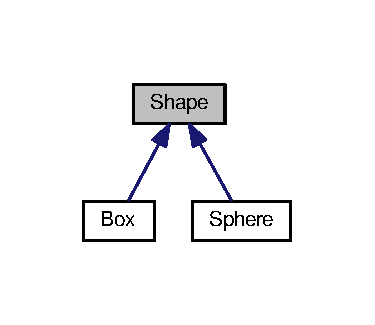
\includegraphics[width=180pt]{class_shape__inherit__graph}
\end{center}
\end{figure}
\subsection*{Public Member Functions}
\begin{DoxyCompactItemize}
\item 
\hyperlink{class_shape_ac88bb6ad20b88fd4d3424ef2f13f20ed}{Shape} (const glm\+::dvec4 \&color, const glm\+::dvec4 \&emissive, const glm\+::dvec4 \&reflect)
\item 
virtual \hyperlink{class_shape_ac3b9fc48965274893f25b18aa14ba665}{$\sim$\+Shape} ()
\item 
virtual \hyperlink{class_shape}{Shape} $\ast$ \hyperlink{class_shape_a99f9bc881b17366992a3edf278b105d0}{copy} () const =0
\item 
virtual std\+::vector$<$ double $>$ \hyperlink{class_shape_aa75a11aaba99bddfccf772faa7e6324b}{intersect} (const \hyperlink{class_ray}{Ray} \&ray) const =0
\item 
virtual glm\+::dvec3 \hyperlink{class_shape_a8444ffb396f26bd86c1c11bc6c47a74d}{normal} (const glm\+::dvec3 \&point) const =0
\item 
glm\+::dvec4 \hyperlink{class_shape_aa6568381e79d7ea3329829253601c64b}{get\+Color} () const 
\item 
glm\+::dvec4 \hyperlink{class_shape_a2e655e8d2e561f0373f3195fa18ec2dd}{get\+Emissive} () const 
\item 
glm\+::dvec4 \hyperlink{class_shape_a999c83a1d16cfa3743d4a117c54bfa00}{get\+Reflect} () const 
\item 
glm\+::dvec4 \hyperlink{class_shape_a51fed50eac9fbb4c39bd226e92643051}{normal\+Color} (const glm\+::dvec3 \&point) const 
\end{DoxyCompactItemize}


\subsection{Constructor \& Destructor Documentation}
\index{Shape@{Shape}!Shape@{Shape}}
\index{Shape@{Shape}!Shape@{Shape}}
\subsubsection[{\texorpdfstring{Shape(const glm\+::dvec4 \&color, const glm\+::dvec4 \&emissive, const glm\+::dvec4 \&reflect)}{Shape(const glm::dvec4 &color, const glm::dvec4 &emissive, const glm::dvec4 &reflect)}}]{\setlength{\rightskip}{0pt plus 5cm}Shape\+::\+Shape (
\begin{DoxyParamCaption}
\item[{const glm\+::dvec4 \&}]{color, }
\item[{const glm\+::dvec4 \&}]{emissive, }
\item[{const glm\+::dvec4 \&}]{reflect}
\end{DoxyParamCaption}
)}\hypertarget{class_shape_ac88bb6ad20b88fd4d3424ef2f13f20ed}{}\label{class_shape_ac88bb6ad20b88fd4d3424ef2f13f20ed}
Construct a shape 
\begin{DoxyParams}{Parameters}
{\em color} & \+: Color of the shape \\
\hline
{\em emissive} & \+: Emissive color of the shape \\
\hline
{\em reflect} & \+: Reflection coefficients of the shape \\
\hline
\end{DoxyParams}
\index{Shape@{Shape}!````~Shape@{$\sim$\+Shape}}
\index{````~Shape@{$\sim$\+Shape}!Shape@{Shape}}
\subsubsection[{\texorpdfstring{$\sim$\+Shape()}{~Shape()}}]{\setlength{\rightskip}{0pt plus 5cm}virtual Shape\+::$\sim$\+Shape (
\begin{DoxyParamCaption}
{}
\end{DoxyParamCaption}
)\hspace{0.3cm}{\ttfamily [inline]}, {\ttfamily [virtual]}}\hypertarget{class_shape_ac3b9fc48965274893f25b18aa14ba665}{}\label{class_shape_ac3b9fc48965274893f25b18aa14ba665}
Destruct the shape 

\subsection{Member Function Documentation}
\index{Shape@{Shape}!copy@{copy}}
\index{copy@{copy}!Shape@{Shape}}
\subsubsection[{\texorpdfstring{copy() const =0}{copy() const =0}}]{\setlength{\rightskip}{0pt plus 5cm}virtual {\bf Shape}$\ast$ Shape\+::copy (
\begin{DoxyParamCaption}
{}
\end{DoxyParamCaption}
) const\hspace{0.3cm}{\ttfamily [pure virtual]}}\hypertarget{class_shape_a99f9bc881b17366992a3edf278b105d0}{}\label{class_shape_a99f9bc881b17366992a3edf278b105d0}
Copy the shape \begin{DoxyReturn}{Returns}
a deep copy of the shape 
\end{DoxyReturn}


Implemented in \hyperlink{class_box_a4770c219ac36060feee72d02c45dab04}{Box}, and \hyperlink{class_sphere_a4510f5adf2bbee77129764097ef48d8a}{Sphere}.

\index{Shape@{Shape}!get\+Color@{get\+Color}}
\index{get\+Color@{get\+Color}!Shape@{Shape}}
\subsubsection[{\texorpdfstring{get\+Color() const }{getColor() const }}]{\setlength{\rightskip}{0pt plus 5cm}glm\+::dvec4 Shape\+::get\+Color (
\begin{DoxyParamCaption}
{}
\end{DoxyParamCaption}
) const}\hypertarget{class_shape_aa6568381e79d7ea3329829253601c64b}{}\label{class_shape_aa6568381e79d7ea3329829253601c64b}
Get the color of the shape \begin{DoxyReturn}{Returns}
the color of the shape 
\end{DoxyReturn}
\index{Shape@{Shape}!get\+Emissive@{get\+Emissive}}
\index{get\+Emissive@{get\+Emissive}!Shape@{Shape}}
\subsubsection[{\texorpdfstring{get\+Emissive() const }{getEmissive() const }}]{\setlength{\rightskip}{0pt plus 5cm}glm\+::dvec4 Shape\+::get\+Emissive (
\begin{DoxyParamCaption}
{}
\end{DoxyParamCaption}
) const}\hypertarget{class_shape_a2e655e8d2e561f0373f3195fa18ec2dd}{}\label{class_shape_a2e655e8d2e561f0373f3195fa18ec2dd}
Get the emissive color of the shape \begin{DoxyReturn}{Returns}
the emissive color of the shape 
\end{DoxyReturn}
\index{Shape@{Shape}!get\+Reflect@{get\+Reflect}}
\index{get\+Reflect@{get\+Reflect}!Shape@{Shape}}
\subsubsection[{\texorpdfstring{get\+Reflect() const }{getReflect() const }}]{\setlength{\rightskip}{0pt plus 5cm}glm\+::dvec4 Shape\+::get\+Reflect (
\begin{DoxyParamCaption}
{}
\end{DoxyParamCaption}
) const}\hypertarget{class_shape_a999c83a1d16cfa3743d4a117c54bfa00}{}\label{class_shape_a999c83a1d16cfa3743d4a117c54bfa00}
Get the reflection coefficients of the shape \begin{DoxyReturn}{Returns}
the reflection coefficients of the shape 
\end{DoxyReturn}
\index{Shape@{Shape}!intersect@{intersect}}
\index{intersect@{intersect}!Shape@{Shape}}
\subsubsection[{\texorpdfstring{intersect(const Ray \&ray) const =0}{intersect(const Ray &ray) const =0}}]{\setlength{\rightskip}{0pt plus 5cm}virtual std\+::vector$<$double$>$ Shape\+::intersect (
\begin{DoxyParamCaption}
\item[{const {\bf Ray} \&}]{ray}
\end{DoxyParamCaption}
) const\hspace{0.3cm}{\ttfamily [pure virtual]}}\hypertarget{class_shape_aa75a11aaba99bddfccf772faa7e6324b}{}\label{class_shape_aa75a11aaba99bddfccf772faa7e6324b}
Get the parametric values on the ray where the shape is intersected

A point on a ray can be written as {\itshape O + tD}, where {\itshape O} is the origin, {\itshape D} the direction and {\itshape t} a scalar. This function will return all values {\itshape t} where the ray hit the shape. If the ray did not hit the shape, the returned vector is empty.


\begin{DoxyParams}{Parameters}
{\em ray} & \+: Tested ray \\
\hline
\end{DoxyParams}
\begin{DoxyReturn}{Returns}
a vector containing all values {\itshape t} where the shape is intersected 
\end{DoxyReturn}


Implemented in \hyperlink{class_box_a32bbf5e25c16d002f2ff858177c25cd8}{Box}, and \hyperlink{class_sphere_afbd74bde6764fe9a037a86c2b38f1fce}{Sphere}.

\index{Shape@{Shape}!normal@{normal}}
\index{normal@{normal}!Shape@{Shape}}
\subsubsection[{\texorpdfstring{normal(const glm\+::dvec3 \&point) const =0}{normal(const glm::dvec3 &point) const =0}}]{\setlength{\rightskip}{0pt plus 5cm}virtual glm\+::dvec3 Shape\+::normal (
\begin{DoxyParamCaption}
\item[{const glm\+::dvec3 \&}]{point}
\end{DoxyParamCaption}
) const\hspace{0.3cm}{\ttfamily [pure virtual]}}\hypertarget{class_shape_a8444ffb396f26bd86c1c11bc6c47a74d}{}\label{class_shape_a8444ffb396f26bd86c1c11bc6c47a74d}
Get the normal of the shape at a particular point

The point have to be on the surface of the shape.


\begin{DoxyParams}{Parameters}
{\em point} & \+: Point where we want to retrieve the normal \\
\hline
\end{DoxyParams}
\begin{DoxyReturn}{Returns}
the normal of the shape 
\end{DoxyReturn}


Implemented in \hyperlink{class_box_a13821ada4849a78e238ced9260904a15}{Box}, and \hyperlink{class_sphere_a9ee72459ad76bddcc1dfb308991b33ee}{Sphere}.

\index{Shape@{Shape}!normal\+Color@{normal\+Color}}
\index{normal\+Color@{normal\+Color}!Shape@{Shape}}
\subsubsection[{\texorpdfstring{normal\+Color(const glm\+::dvec3 \&point) const }{normalColor(const glm::dvec3 &point) const }}]{\setlength{\rightskip}{0pt plus 5cm}glm\+::dvec4 Shape\+::normal\+Color (
\begin{DoxyParamCaption}
\item[{const glm\+::dvec3 \&}]{point}
\end{DoxyParamCaption}
) const}\hypertarget{class_shape_a51fed50eac9fbb4c39bd226e92643051}{}\label{class_shape_a51fed50eac9fbb4c39bd226e92643051}
Get the normal as a color of the shape at a particular point

This function is used for debugging purpose.

\begin{DoxyReturn}{Returns}
the normal of the shape as a color 
\end{DoxyReturn}


The documentation for this class was generated from the following file\+:\begin{DoxyCompactItemize}
\item 
include/\hyperlink{shape_8hpp}{shape.\+hpp}\end{DoxyCompactItemize}

\hypertarget{class_sphere}{}\section{Sphere Class Reference}
\label{class_sphere}\index{Sphere@{Sphere}}


Class representing a sphere in the scene.  




{\ttfamily \#include $<$sphere.\+hpp$>$}



Inheritance diagram for Sphere\+:
\nopagebreak
\begin{figure}[H]
\begin{center}
\leavevmode
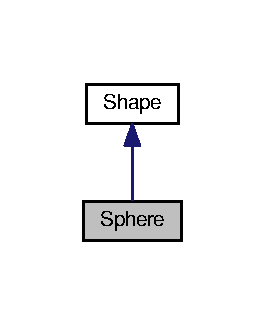
\includegraphics[width=127pt]{class_sphere__inherit__graph}
\end{center}
\end{figure}


Collaboration diagram for Sphere\+:
\nopagebreak
\begin{figure}[H]
\begin{center}
\leavevmode
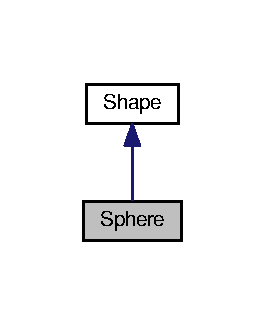
\includegraphics[width=127pt]{class_sphere__coll__graph}
\end{center}
\end{figure}
\subsection*{Public Member Functions}
\begin{DoxyCompactItemize}
\item 
\hyperlink{class_sphere_a4e8ff9197b7acbecd4b1f40106ebd2cf}{Sphere} (const glm\+::dvec3 \&center, double radius, const glm\+::dvec4 \&color, const glm\+::dvec4 \&emissive, const glm\+::dvec4 \&reflect)
\item 
\hyperlink{class_shape}{Shape} $\ast$ \hyperlink{class_sphere_a4510f5adf2bbee77129764097ef48d8a}{copy} () const 
\item 
std\+::vector$<$ double $>$ \hyperlink{class_sphere_afbd74bde6764fe9a037a86c2b38f1fce}{intersect} (const \hyperlink{class_ray}{Ray} \&ray) const override
\item 
glm\+::dvec3 \hyperlink{class_sphere_a9ee72459ad76bddcc1dfb308991b33ee}{normal} (const glm\+::dvec3 \&point) const override
\end{DoxyCompactItemize}


\subsection{Detailed Description}
Class representing a sphere in the scene. 

\subsection{Constructor \& Destructor Documentation}
\index{Sphere@{Sphere}!Sphere@{Sphere}}
\index{Sphere@{Sphere}!Sphere@{Sphere}}
\subsubsection[{\texorpdfstring{Sphere(const glm\+::dvec3 \&center, double radius, const glm\+::dvec4 \&color, const glm\+::dvec4 \&emissive, const glm\+::dvec4 \&reflect)}{Sphere(const glm::dvec3 &center, double radius, const glm::dvec4 &color, const glm::dvec4 &emissive, const glm::dvec4 &reflect)}}]{\setlength{\rightskip}{0pt plus 5cm}Sphere\+::\+Sphere (
\begin{DoxyParamCaption}
\item[{const glm\+::dvec3 \&}]{center, }
\item[{double}]{radius, }
\item[{const glm\+::dvec4 \&}]{color, }
\item[{const glm\+::dvec4 \&}]{emissive, }
\item[{const glm\+::dvec4 \&}]{reflect}
\end{DoxyParamCaption}
)\hspace{0.3cm}{\ttfamily [explicit]}}\hypertarget{class_sphere_a4e8ff9197b7acbecd4b1f40106ebd2cf}{}\label{class_sphere_a4e8ff9197b7acbecd4b1f40106ebd2cf}
Construct a sphere 
\begin{DoxyParams}{Parameters}
{\em center} & \+: Center of the sphere \\
\hline
{\em radius} & \+: Radius of the sphere \\
\hline
{\em color} & \+: Color of the sphere \\
\hline
{\em emissive} & \+: Emissive color of the sphere \\
\hline
{\em reflect} & \+: Reflection coefficients of the sphere \\
\hline
\end{DoxyParams}


\subsection{Member Function Documentation}
\index{Sphere@{Sphere}!copy@{copy}}
\index{copy@{copy}!Sphere@{Sphere}}
\subsubsection[{\texorpdfstring{copy() const }{copy() const }}]{\setlength{\rightskip}{0pt plus 5cm}{\bf Shape}$\ast$ Sphere\+::copy (
\begin{DoxyParamCaption}
{}
\end{DoxyParamCaption}
) const\hspace{0.3cm}{\ttfamily [virtual]}}\hypertarget{class_sphere_a4510f5adf2bbee77129764097ef48d8a}{}\label{class_sphere_a4510f5adf2bbee77129764097ef48d8a}
Copy the sphere \begin{DoxyReturn}{Returns}
a deep copy of the sphere 
\end{DoxyReturn}


Implements \hyperlink{class_shape_a99f9bc881b17366992a3edf278b105d0}{Shape}.

\index{Sphere@{Sphere}!intersect@{intersect}}
\index{intersect@{intersect}!Sphere@{Sphere}}
\subsubsection[{\texorpdfstring{intersect(const Ray \&ray) const override}{intersect(const Ray &ray) const override}}]{\setlength{\rightskip}{0pt plus 5cm}std\+::vector$<$double$>$ Sphere\+::intersect (
\begin{DoxyParamCaption}
\item[{const {\bf Ray} \&}]{ray}
\end{DoxyParamCaption}
) const\hspace{0.3cm}{\ttfamily [override]}, {\ttfamily [virtual]}}\hypertarget{class_sphere_afbd74bde6764fe9a037a86c2b38f1fce}{}\label{class_sphere_afbd74bde6764fe9a037a86c2b38f1fce}
Get the parametric values on the ray where the sphere is intersected

A point on a ray can be written as {\itshape O + tD}, where {\itshape O} is the origin, {\itshape D} the direction and {\itshape t} a scalar. This function will return all values {\itshape t} where the ray hit the sphere. If the ray did not hit the sphere, the returned vector is empty.


\begin{DoxyParams}{Parameters}
{\em ray} & Tested ray \\
\hline
\end{DoxyParams}
\begin{DoxyReturn}{Returns}
a vector containing all values {\itshape t} where the sphere is intersected 
\end{DoxyReturn}


Implements \hyperlink{class_shape_aa75a11aaba99bddfccf772faa7e6324b}{Shape}.

\index{Sphere@{Sphere}!normal@{normal}}
\index{normal@{normal}!Sphere@{Sphere}}
\subsubsection[{\texorpdfstring{normal(const glm\+::dvec3 \&point) const override}{normal(const glm::dvec3 &point) const override}}]{\setlength{\rightskip}{0pt plus 5cm}glm\+::dvec3 Sphere\+::normal (
\begin{DoxyParamCaption}
\item[{const glm\+::dvec3 \&}]{point}
\end{DoxyParamCaption}
) const\hspace{0.3cm}{\ttfamily [override]}, {\ttfamily [virtual]}}\hypertarget{class_sphere_a9ee72459ad76bddcc1dfb308991b33ee}{}\label{class_sphere_a9ee72459ad76bddcc1dfb308991b33ee}
Get the normal of the sphere at a particular point

The point have to be on the surface of the sphere.


\begin{DoxyParams}{Parameters}
{\em point} & Point where we want to retrieve the normal \\
\hline
\end{DoxyParams}
\begin{DoxyReturn}{Returns}
the normal of the sphere 
\end{DoxyReturn}


Implements \hyperlink{class_shape_a8444ffb396f26bd86c1c11bc6c47a74d}{Shape}.



The documentation for this class was generated from the following file\+:\begin{DoxyCompactItemize}
\item 
include/\hyperlink{sphere_8hpp}{sphere.\+hpp}\end{DoxyCompactItemize}

\chapter{File Documentation}
\hypertarget{box_8hpp}{}\section{include/box.hpp File Reference}
\label{box_8hpp}\index{include/box.\+hpp@{include/box.\+hpp}}


Representation of box.  


{\ttfamily \#include \char`\"{}shape.\+hpp\char`\"{}}\\*
{\ttfamily \#include \char`\"{}ray.\+hpp\char`\"{}}\\*
{\ttfamily \#include $<$glm/glm.\+hpp$>$}\\*
{\ttfamily \#include $<$vector$>$}\\*
Include dependency graph for box.\+hpp\+:
\nopagebreak
\begin{figure}[H]
\begin{center}
\leavevmode
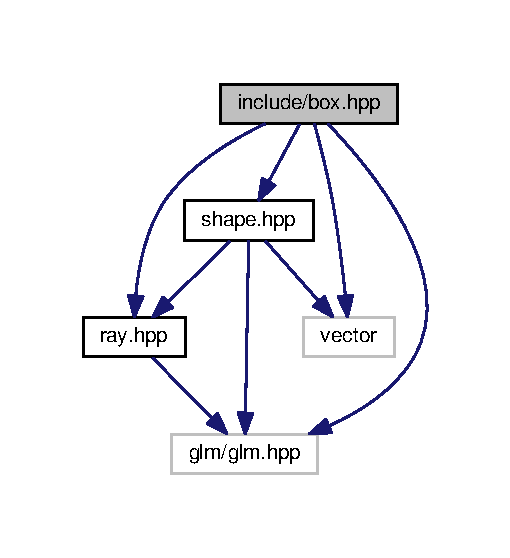
\includegraphics[width=245pt]{box_8hpp__incl}
\end{center}
\end{figure}
This graph shows which files directly or indirectly include this file\+:
\nopagebreak
\begin{figure}[H]
\begin{center}
\leavevmode
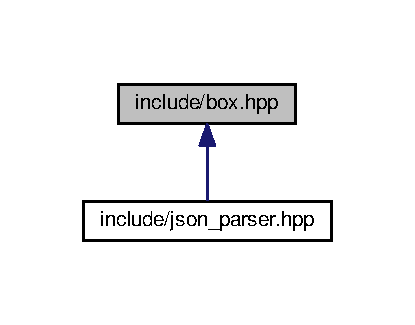
\includegraphics[width=199pt]{box_8hpp__dep__incl}
\end{center}
\end{figure}
\subsection*{Classes}
\begin{DoxyCompactItemize}
\item 
class \hyperlink{class_box}{Box}
\begin{DoxyCompactList}\small\item\em Class representing a box in the scene. \end{DoxyCompactList}\end{DoxyCompactItemize}


\subsection{Detailed Description}
Representation of box. 

Representation of collision point.

Module for manipulation of boxes.

Module for manipulation of collision points. The collision points are used to compute the intersection between a ray and a shape of the scene. 
\hypertarget{camera_8hpp}{}\section{include/camera.hpp File Reference}
\label{camera_8hpp}\index{include/camera.\+hpp@{include/camera.\+hpp}}


Representation of camera.  


{\ttfamily \#include $<$glm/glm.\+hpp$>$}\\*
Include dependency graph for camera.\+hpp\+:
\nopagebreak
\begin{figure}[H]
\begin{center}
\leavevmode
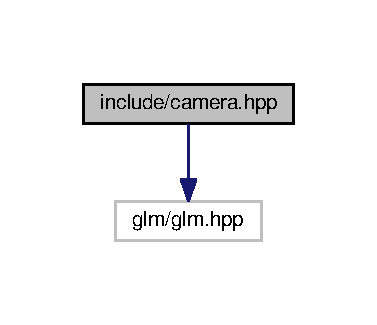
\includegraphics[width=181pt]{camera_8hpp__incl}
\end{center}
\end{figure}
This graph shows which files directly or indirectly include this file\+:
\nopagebreak
\begin{figure}[H]
\begin{center}
\leavevmode
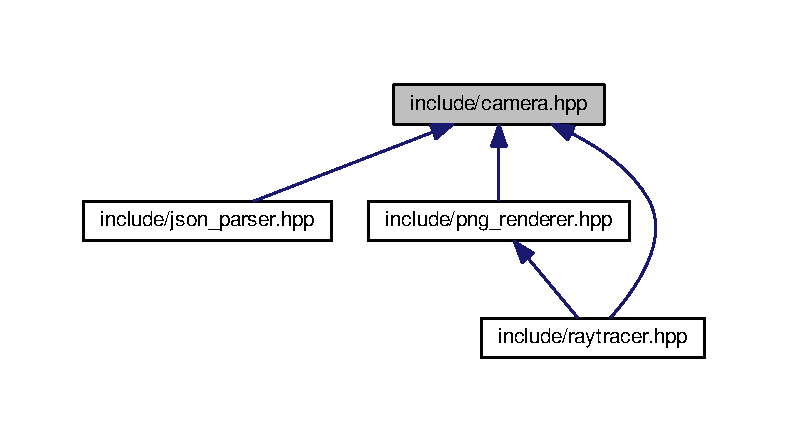
\includegraphics[width=350pt]{camera_8hpp__dep__incl}
\end{center}
\end{figure}
\subsection*{Classes}
\begin{DoxyCompactItemize}
\item 
class \hyperlink{class_camera}{Camera}
\begin{DoxyCompactList}\small\item\em Class representing a camera. \end{DoxyCompactList}\end{DoxyCompactItemize}


\subsection{Detailed Description}
Representation of camera. 

Module for manipulation of cameras. 
\hypertarget{json__parser_8hpp}{}\section{include/json\+\_\+parser.hpp File Reference}
\label{json__parser_8hpp}\index{include/json\+\_\+parser.\+hpp@{include/json\+\_\+parser.\+hpp}}


Methods to parse J\+S\+ON files.  


{\ttfamily \#include \char`\"{}scene.\+hpp\char`\"{}}\\*
{\ttfamily \#include \char`\"{}camera.\+hpp\char`\"{}}\\*
{\ttfamily \#include \char`\"{}shape.\+hpp\char`\"{}}\\*
{\ttfamily \#include \char`\"{}sphere.\+hpp\char`\"{}}\\*
{\ttfamily \#include \char`\"{}box.\+hpp\char`\"{}}\\*
{\ttfamily \#include \char`\"{}light.\+hpp\char`\"{}}\\*
{\ttfamily \#include $<$json/json.\+hpp$>$}\\*
{\ttfamily \#include $<$string$>$}\\*
{\ttfamily \#include $<$utility$>$}\\*
{\ttfamily \#include $<$glm/glm.\+hpp$>$}\\*
{\ttfamily \#include $<$glm/gtc/type\+\_\+ptr.\+hpp$>$}\\*
Include dependency graph for json\+\_\+parser.\+hpp\+:
\nopagebreak
\begin{figure}[H]
\begin{center}
\leavevmode
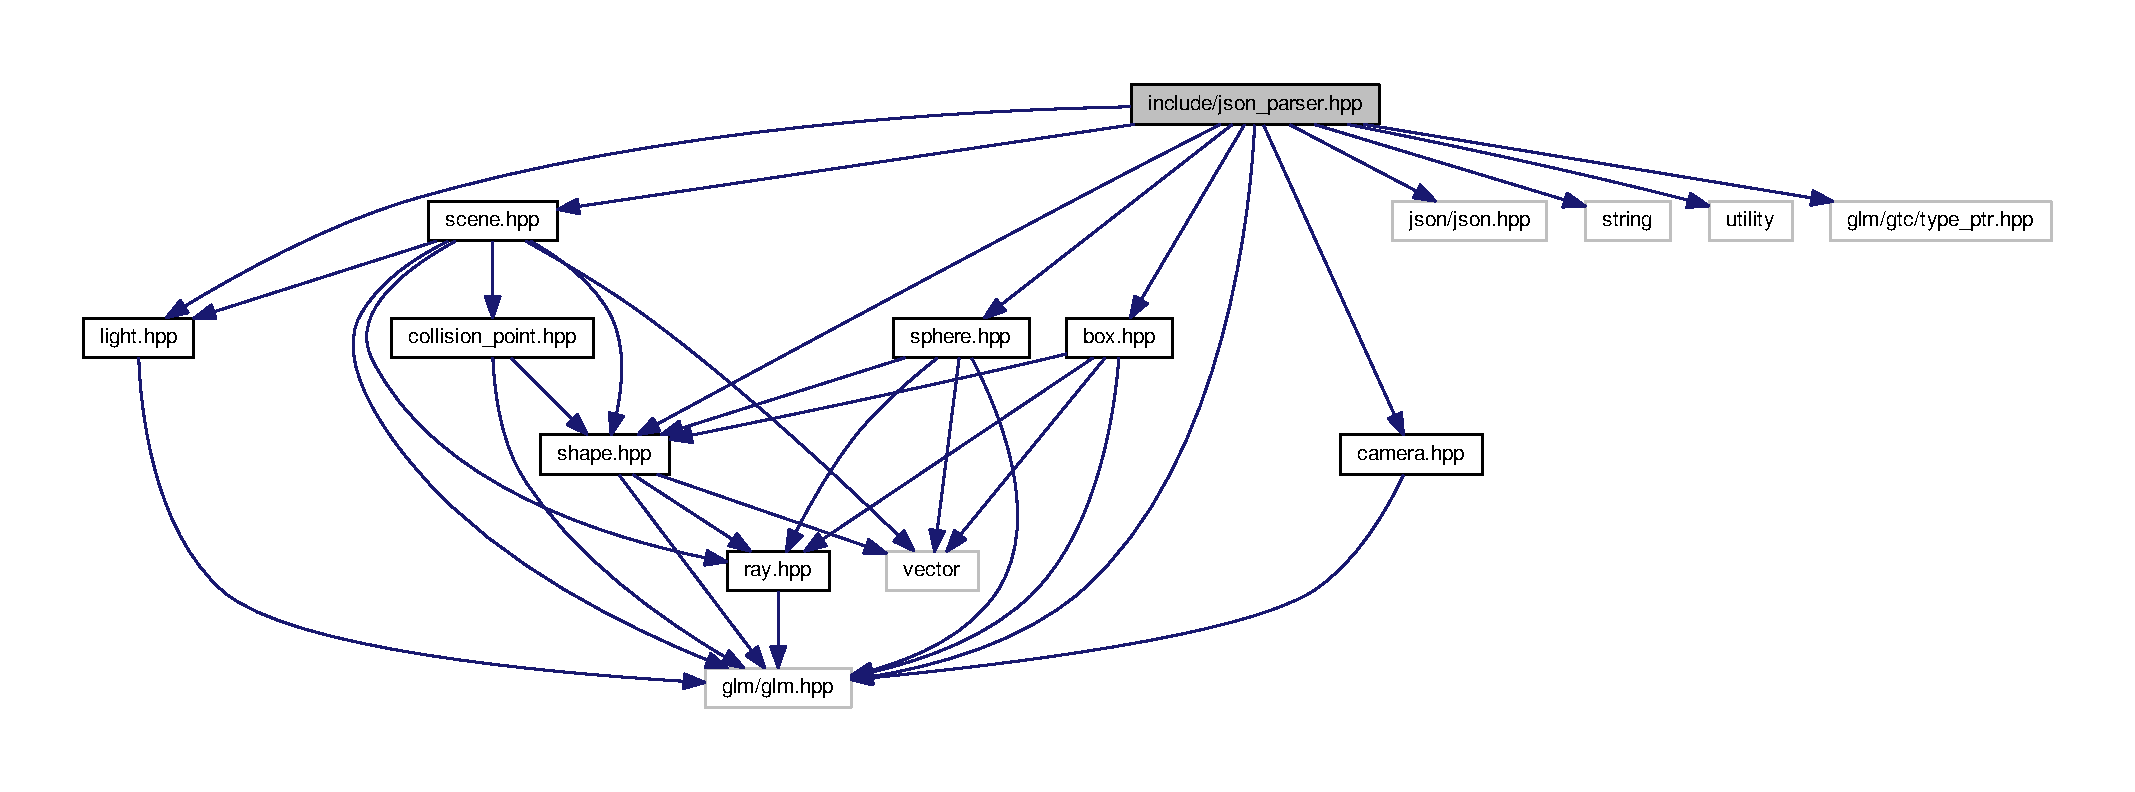
\includegraphics[width=350pt]{json__parser_8hpp__incl}
\end{center}
\end{figure}
\subsection*{Classes}
\begin{DoxyCompactItemize}
\item 
class \hyperlink{class_j_s_o_n_parser}{J\+S\+O\+N\+Parser}
\begin{DoxyCompactList}\small\item\em Helper class to parse the J\+S\+ON scene files. \end{DoxyCompactList}\end{DoxyCompactItemize}
\subsection*{Typedefs}
\begin{DoxyCompactItemize}
\item 
using {\bfseries json} = nlohmann\+::json\hypertarget{json__parser_8hpp_ab701e3ac61a85b337ec5c1abaad6742d}{}\label{json__parser_8hpp_ab701e3ac61a85b337ec5c1abaad6742d}

\end{DoxyCompactItemize}


\subsection{Detailed Description}
Methods to parse J\+S\+ON files. 

Module that provide the functions to parse J\+S\+ON representation of displayable scene. 
\hypertarget{light_8hpp}{}\section{include/light.hpp File Reference}
\label{light_8hpp}\index{include/light.\+hpp@{include/light.\+hpp}}


Representation of light.  


{\ttfamily \#include $<$glm/glm.\+hpp$>$}\\*
Include dependency graph for light.\+hpp\+:
\nopagebreak
\begin{figure}[H]
\begin{center}
\leavevmode
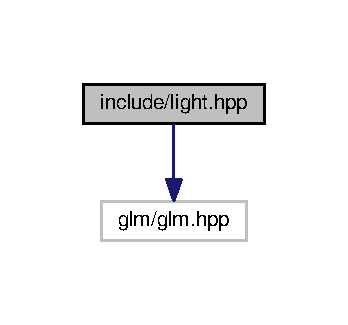
\includegraphics[width=167pt]{light_8hpp__incl}
\end{center}
\end{figure}
This graph shows which files directly or indirectly include this file\+:
\nopagebreak
\begin{figure}[H]
\begin{center}
\leavevmode
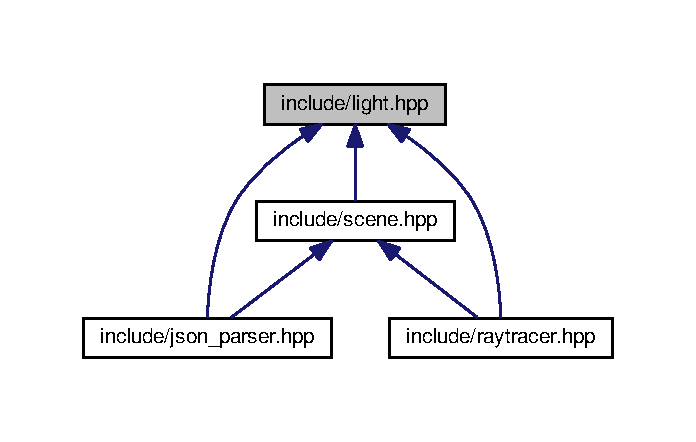
\includegraphics[width=334pt]{light_8hpp__dep__incl}
\end{center}
\end{figure}
\subsection*{Classes}
\begin{DoxyCompactItemize}
\item 
class \hyperlink{class_light}{Light}
\begin{DoxyCompactList}\small\item\em Class representing a light in the scene. \end{DoxyCompactList}\end{DoxyCompactItemize}


\subsection{Detailed Description}
Representation of light. 

Module for manipulation of lights. 
\hypertarget{png__renderer_8hpp}{}\section{include/png\+\_\+renderer.hpp File Reference}
\label{png__renderer_8hpp}\index{include/png\+\_\+renderer.\+hpp@{include/png\+\_\+renderer.\+hpp}}


Methods to render the result.  


{\ttfamily \#include \char`\"{}camera.\+hpp\char`\"{}}\\*
{\ttfamily \#include $<$glm/glm.\+hpp$>$}\\*
{\ttfamily \#include $<$string$>$}\\*
Include dependency graph for png\+\_\+renderer.\+hpp\+:
\nopagebreak
\begin{figure}[H]
\begin{center}
\leavevmode
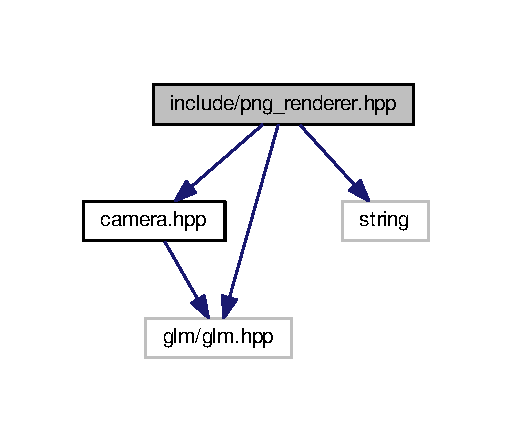
\includegraphics[width=246pt]{png__renderer_8hpp__incl}
\end{center}
\end{figure}
This graph shows which files directly or indirectly include this file\+:
\nopagebreak
\begin{figure}[H]
\begin{center}
\leavevmode
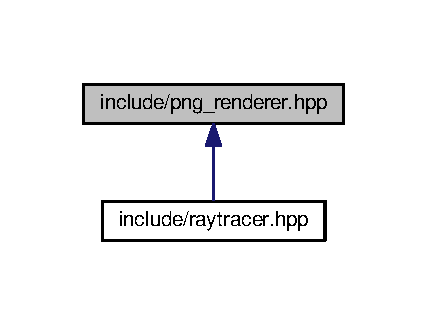
\includegraphics[width=205pt]{png__renderer_8hpp__dep__incl}
\end{center}
\end{figure}
\subsection*{Classes}
\begin{DoxyCompactItemize}
\item 
class \hyperlink{class_p_n_g_renderer}{P\+N\+G\+Renderer}
\begin{DoxyCompactList}\small\item\em Helper class to save the result as a {\itshape }.png file. \end{DoxyCompactList}\end{DoxyCompactItemize}


\subsection{Detailed Description}
Methods to render the result. 

Module that provide a method to save the result. Here we choose to save as a {\itshape }.png file but we can imagine an other renderer that for example display the result in a S\+DL window. 
\hypertarget{ray_8hpp}{}\section{include/ray.hpp File Reference}
\label{ray_8hpp}\index{include/ray.\+hpp@{include/ray.\+hpp}}


Representation of ray.  


{\ttfamily \#include $<$glm/glm.\+hpp$>$}\\*
Include dependency graph for ray.\+hpp\+:
\nopagebreak
\begin{figure}[H]
\begin{center}
\leavevmode
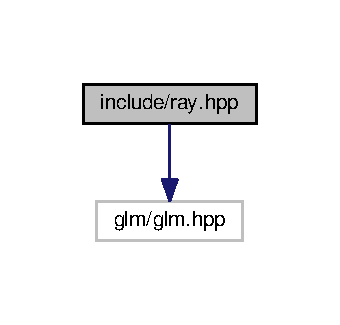
\includegraphics[width=163pt]{ray_8hpp__incl}
\end{center}
\end{figure}
This graph shows which files directly or indirectly include this file\+:
\nopagebreak
\begin{figure}[H]
\begin{center}
\leavevmode
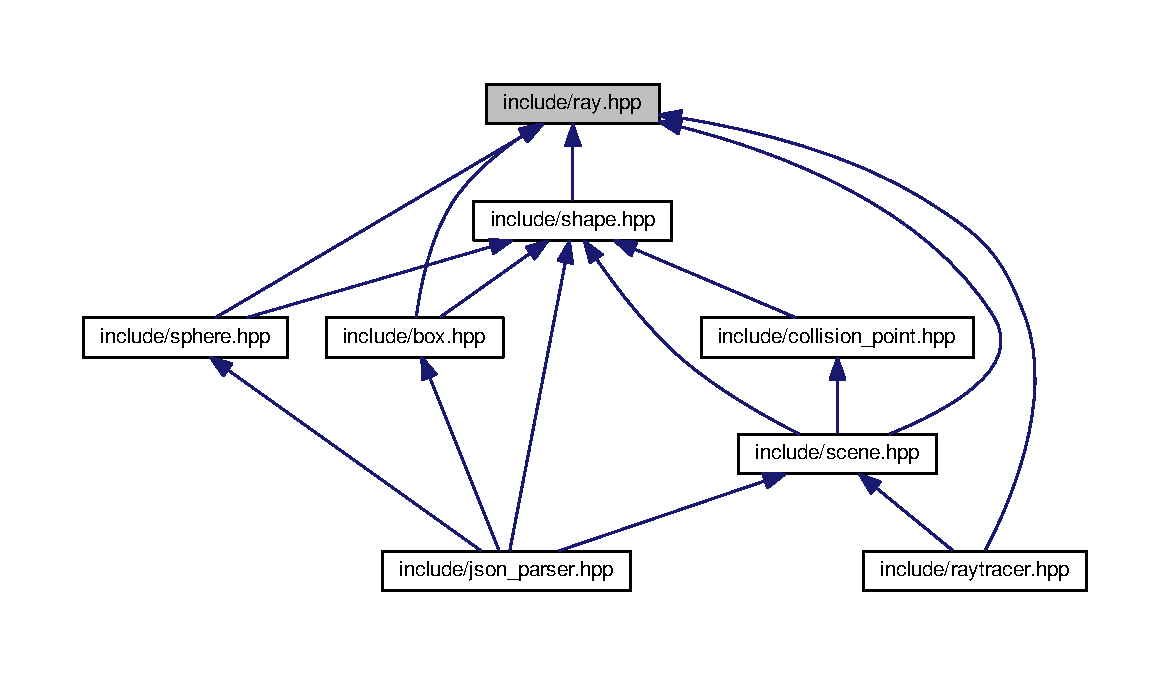
\includegraphics[width=350pt]{ray_8hpp__dep__incl}
\end{center}
\end{figure}
\subsection*{Classes}
\begin{DoxyCompactItemize}
\item 
class \hyperlink{class_ray}{Ray}
\begin{DoxyCompactList}\small\item\em Class representing a ray. \end{DoxyCompactList}\end{DoxyCompactItemize}


\subsection{Detailed Description}
Representation of ray. 

Module for manipulation of rays. 
\hypertarget{raytracer_8hpp}{}\section{include/raytracer.hpp File Reference}
\label{raytracer_8hpp}\index{include/raytracer.\+hpp@{include/raytracer.\+hpp}}


Methods to compute the raytracing.  


{\ttfamily \#include \char`\"{}scene.\+hpp\char`\"{}}\\*
{\ttfamily \#include \char`\"{}camera.\+hpp\char`\"{}}\\*
{\ttfamily \#include \char`\"{}light.\+hpp\char`\"{}}\\*
{\ttfamily \#include \char`\"{}ray.\+hpp\char`\"{}}\\*
{\ttfamily \#include \char`\"{}png\+\_\+renderer.\+hpp\char`\"{}}\\*
{\ttfamily \#include $<$glm/glm.\+hpp$>$}\\*
Include dependency graph for raytracer.\+hpp\+:
\nopagebreak
\begin{figure}[H]
\begin{center}
\leavevmode
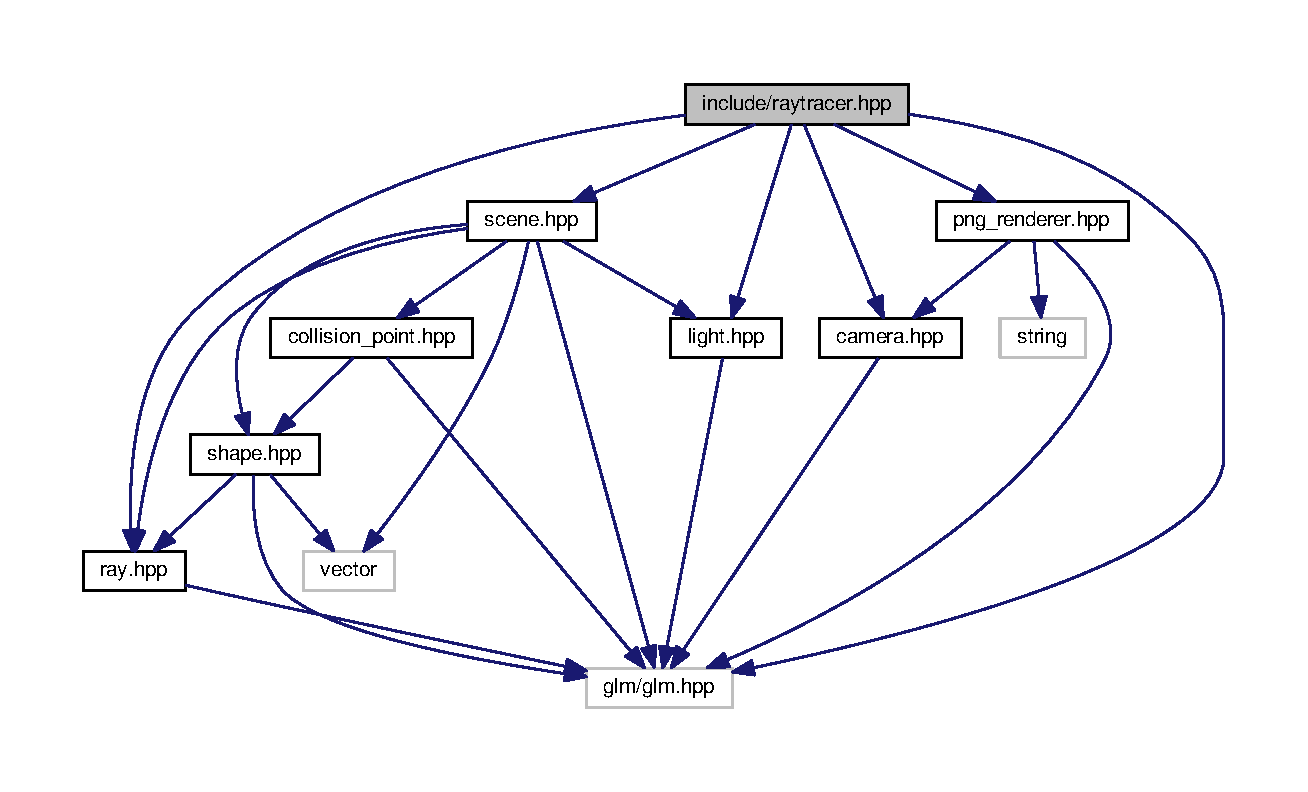
\includegraphics[width=350pt]{raytracer_8hpp__incl}
\end{center}
\end{figure}
\subsection*{Classes}
\begin{DoxyCompactItemize}
\item 
class \hyperlink{class_raytracer}{Raytracer}
\begin{DoxyCompactList}\small\item\em Helper class to compute the result of the ray tracing. \end{DoxyCompactList}\end{DoxyCompactItemize}


\subsection{Detailed Description}
Methods to compute the raytracing. 

Module that provide the ray tracing function. 
\hypertarget{scene_8hpp}{}\section{include/scene.hpp File Reference}
\label{scene_8hpp}\index{include/scene.\+hpp@{include/scene.\+hpp}}


Representation of scene.  


{\ttfamily \#include \char`\"{}shape.\+hpp\char`\"{}}\\*
{\ttfamily \#include \char`\"{}light.\+hpp\char`\"{}}\\*
{\ttfamily \#include \char`\"{}ray.\+hpp\char`\"{}}\\*
{\ttfamily \#include \char`\"{}collision\+\_\+point.\+hpp\char`\"{}}\\*
{\ttfamily \#include $<$vector$>$}\\*
{\ttfamily \#include $<$glm/glm.\+hpp$>$}\\*
Include dependency graph for scene.\+hpp\+:
\nopagebreak
\begin{figure}[H]
\begin{center}
\leavevmode
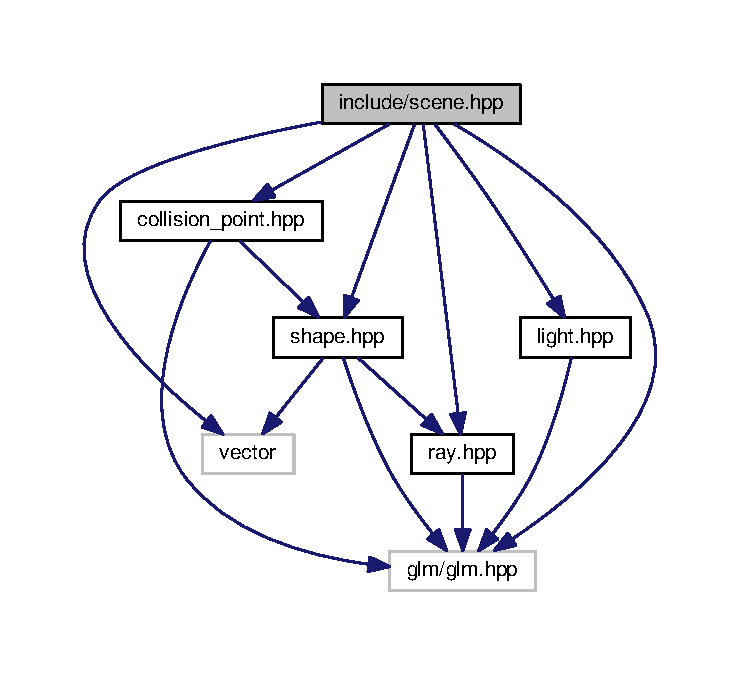
\includegraphics[width=350pt]{scene_8hpp__incl}
\end{center}
\end{figure}
This graph shows which files directly or indirectly include this file\+:
\nopagebreak
\begin{figure}[H]
\begin{center}
\leavevmode
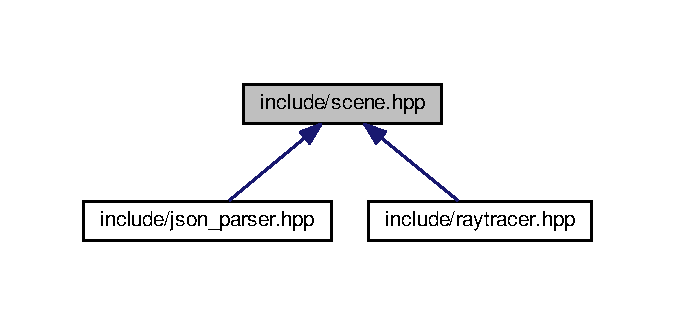
\includegraphics[width=324pt]{scene_8hpp__dep__incl}
\end{center}
\end{figure}
\subsection*{Classes}
\begin{DoxyCompactItemize}
\item 
class \hyperlink{class_scene}{Scene}
\begin{DoxyCompactList}\small\item\em Class representing a scene. \end{DoxyCompactList}\end{DoxyCompactItemize}


\subsection{Detailed Description}
Representation of scene. 

Module for manipulation of scene. 
\hypertarget{shape_8hpp}{}\section{include/shape.hpp File Reference}
\label{shape_8hpp}\index{include/shape.\+hpp@{include/shape.\+hpp}}


Representation of shape.  


{\ttfamily \#include \char`\"{}ray.\+hpp\char`\"{}}\\*
{\ttfamily \#include $<$glm/glm.\+hpp$>$}\\*
{\ttfamily \#include $<$vector$>$}\\*
Include dependency graph for shape.\+hpp\+:
\nopagebreak
\begin{figure}[H]
\begin{center}
\leavevmode
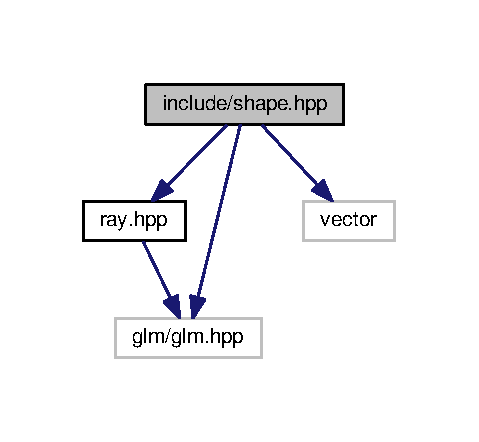
\includegraphics[width=230pt]{shape_8hpp__incl}
\end{center}
\end{figure}
This graph shows which files directly or indirectly include this file\+:
\nopagebreak
\begin{figure}[H]
\begin{center}
\leavevmode
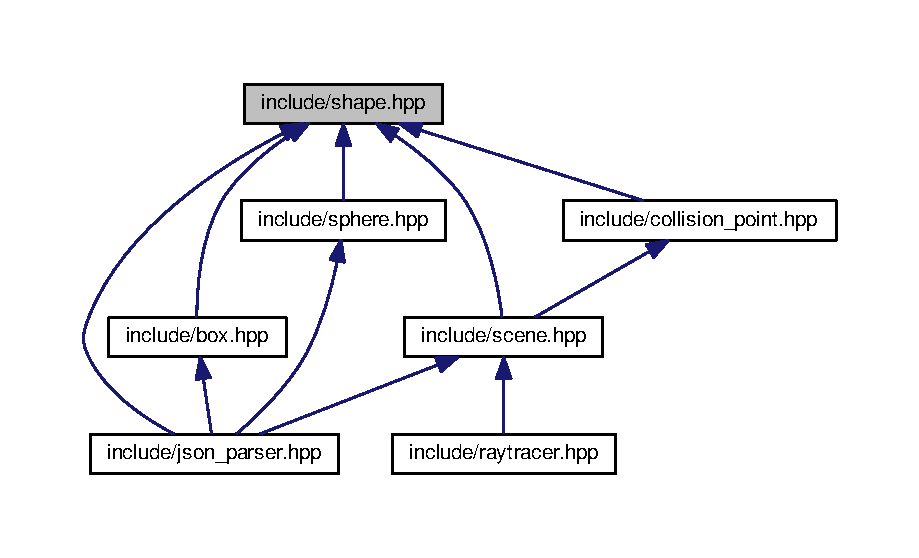
\includegraphics[width=350pt]{shape_8hpp__dep__incl}
\end{center}
\end{figure}
\subsection*{Classes}
\begin{DoxyCompactItemize}
\item 
class \hyperlink{class_shape}{Shape}
\end{DoxyCompactItemize}


\subsection{Detailed Description}
Representation of shape. 

Module for manipulation of shapes. 
\hypertarget{sphere_8hpp}{}\section{include/sphere.hpp File Reference}
\label{sphere_8hpp}\index{include/sphere.\+hpp@{include/sphere.\+hpp}}


Representation of sphere.  


{\ttfamily \#include \char`\"{}shape.\+hpp\char`\"{}}\\*
{\ttfamily \#include \char`\"{}ray.\+hpp\char`\"{}}\\*
{\ttfamily \#include $<$glm/glm.\+hpp$>$}\\*
{\ttfamily \#include $<$vector$>$}\\*
Include dependency graph for sphere.\+hpp\+:
\nopagebreak
\begin{figure}[H]
\begin{center}
\leavevmode
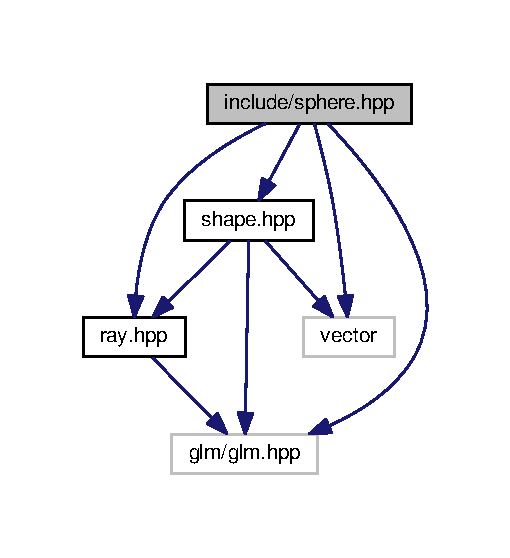
\includegraphics[width=245pt]{sphere_8hpp__incl}
\end{center}
\end{figure}
This graph shows which files directly or indirectly include this file\+:
\nopagebreak
\begin{figure}[H]
\begin{center}
\leavevmode
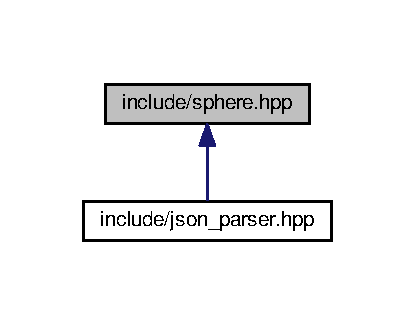
\includegraphics[width=199pt]{sphere_8hpp__dep__incl}
\end{center}
\end{figure}
\subsection*{Classes}
\begin{DoxyCompactItemize}
\item 
class \hyperlink{class_sphere}{Sphere}
\begin{DoxyCompactList}\small\item\em Class representing a sphere in the scene. \end{DoxyCompactList}\end{DoxyCompactItemize}


\subsection{Detailed Description}
Representation of sphere. 

Module for manipulation of spheres. 
%--- End generated contents ---

% Index
\backmatter
\newpage
\phantomsection
\clearemptydoublepage
\addcontentsline{toc}{chapter}{Index}
\printindex

\end{document}
